\chapter{Proposition de modèle de machine learning}
\label{chap:proposition_modele}

Ce chapitre va explorer la création d'un modèle de machine learning de A à Z.

\localtableofcontents

\newpage

% -----------------------------------------------------------------------------
% -----------------------------------------------------------------------------
\section{Introduction}
La création d'un modèle de machine learning implique plusieurs phases. La Figure \ref{fig:ch3_resume_machine_learning_supervise} résume les principales étapes et servira de fil conducteur pour le chapitre.
\begin{figure}[H]
    \centering
    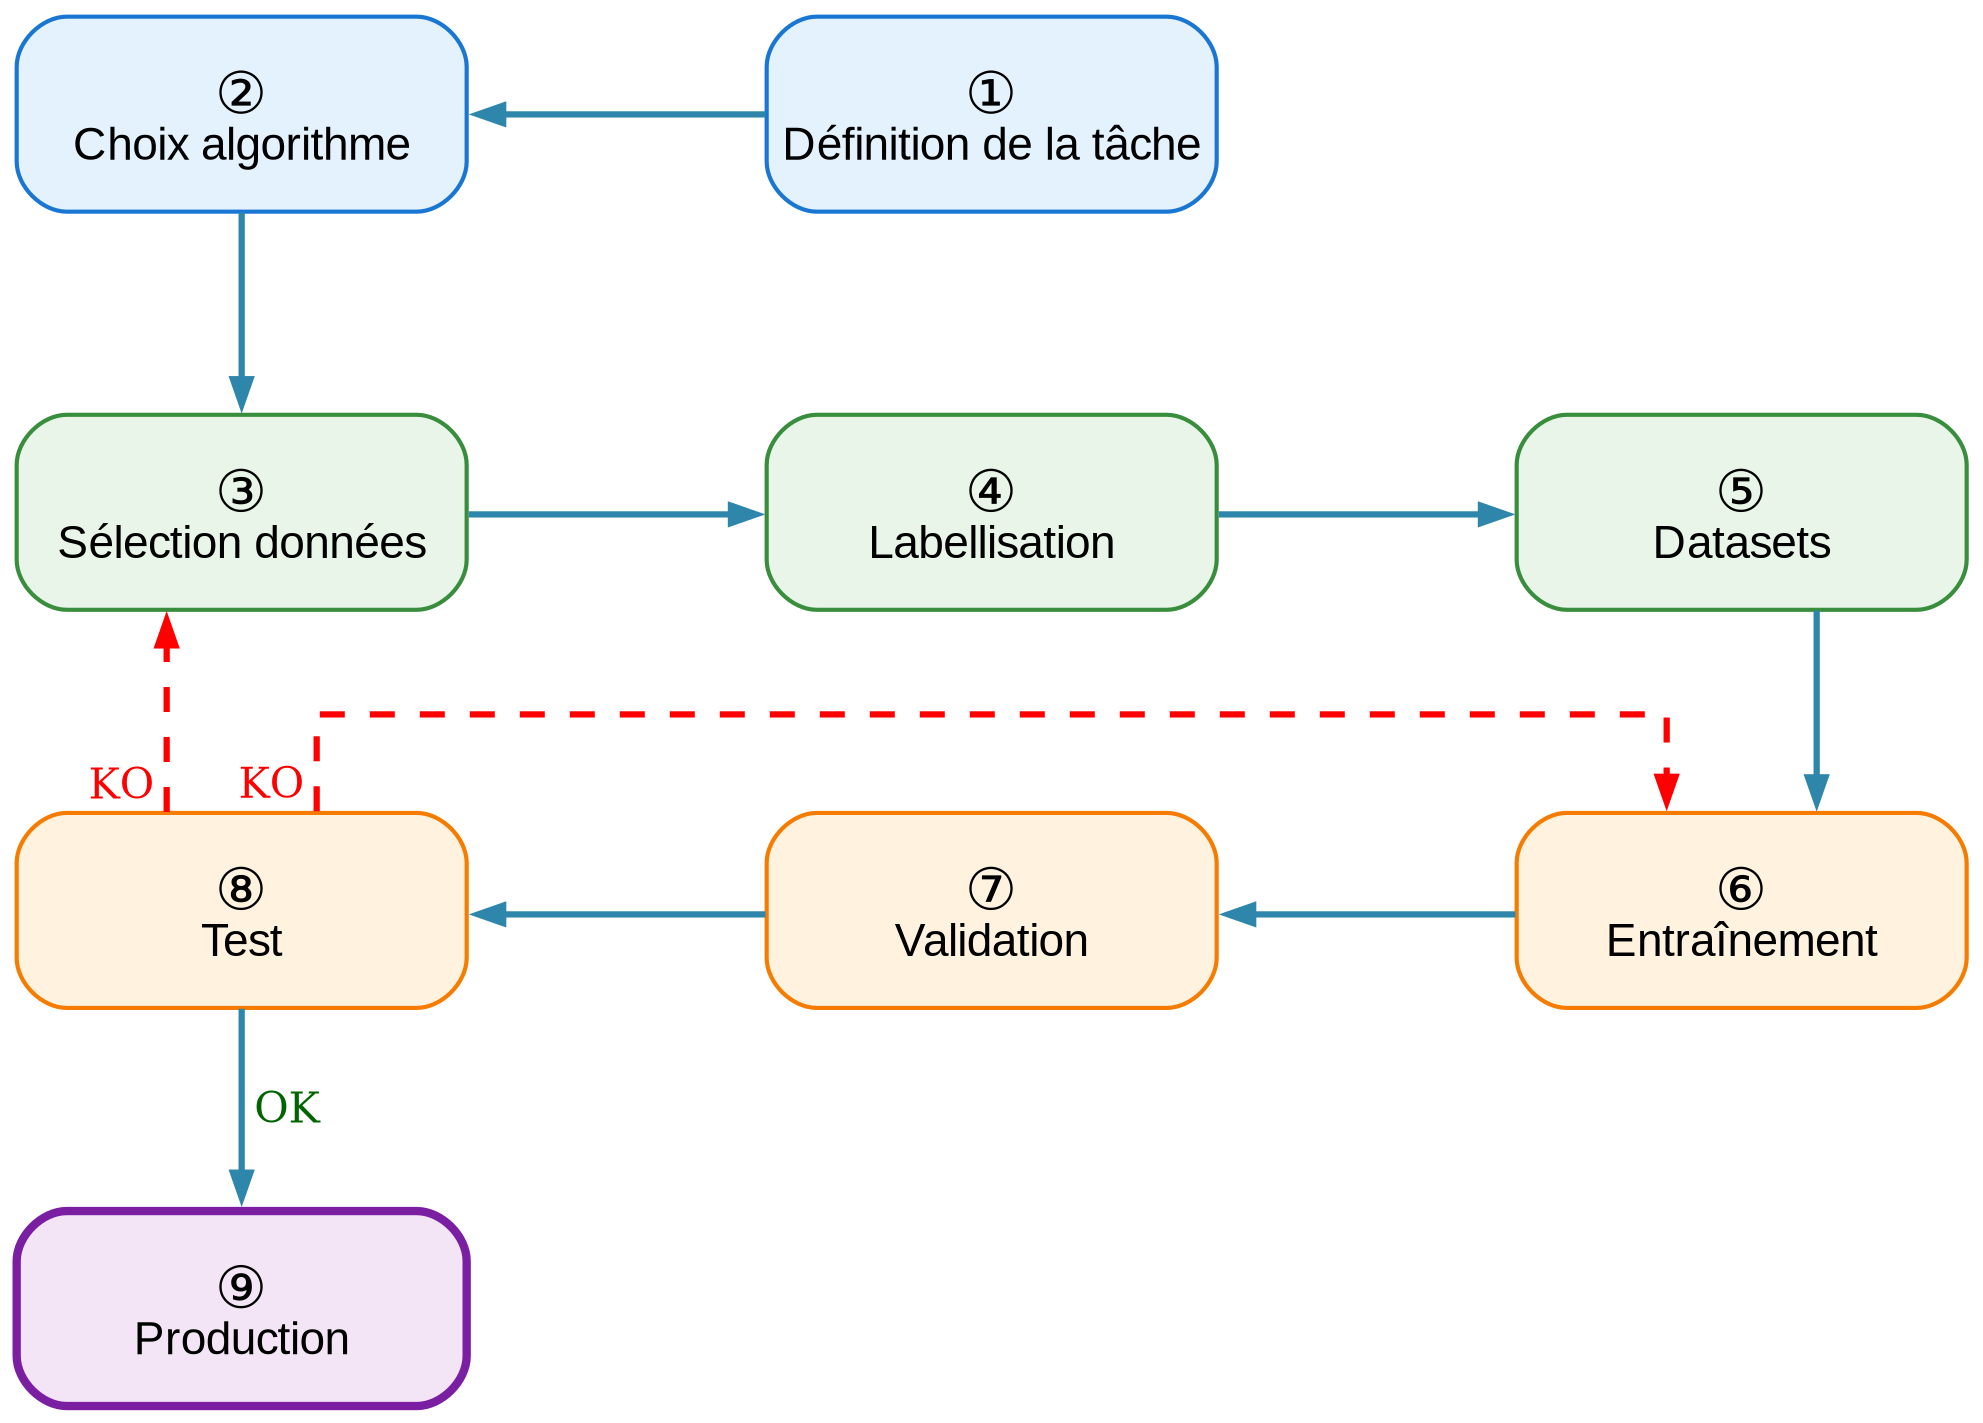
\includegraphics[width=1\linewidth]{03-tail/A1_fondamentaux_ML/A1_figures/A1_01_resume_machine_learning_supervise.png}
    \caption{Résumé de machine learning supervisé}
    \label{fig:ch3_resume_machine_learning_supervise}
\end{figure}
En premier, il faut définir la tâche et choisir le bon algorithme. En deuxième, selon les besoins en données, il faut créer un dataset pour entraîner le modèle. Finalement, lorsque le modèle est suffisamment performant, il peut être utilisé en production. L'Annexe \ref{chap:fondamentaux_ml} permet de se familiariser avec l'ensemble des termes et concepts de machine learning utilisés dans ce chapitre.

Ensuite, une section est dédiée à toutes les pistes explorées qui n'ont pas été retenues. Cette phase nécessaire dans tout projet de recherche doit être valorisée, elle aide à comprendre le cheminement vers une solution viable. Pour conclure le chapitre, les points-clés de ce chapitre seront résumés dans une synthèse.



% -----------------------------------------------------------------------------
% -----------------------------------------------------------------------------
\section{Phase préparatoire}
Cette phase préparatoire intègre les 2 premières étapes de la Figure \ref{fig:ch3_resume_machine_learning_supervise}, c'est-à-dire la définition de la tâche à accomplir et le choix de l'algorithme.

\subsection{Tâche}
La tâche que ce modèle doit accomplir est d'identifier les espaces disponibles sur les toitures. Cette tâche est identique à celle de \acrshort{stdl} du chapitre \ref{subsec:stdl_analyse}, par contre l'approche utilisée va être différente.

\subsection{Algorithme}
Une fois la tâche définie, il faut déterminer une approche. \acrshort{stdl} a exploré 3 approches différentes:
\begin{itemize}
    \item La classification des pans de toit
    \item La segmentation des données \gls{lidar}
    \item La segmentation d'images
\end{itemize}

Leur segmentation d'images est réalisée avec Segment Anything Model (SAM). SAM effectue de la segmentation instance et divise l'image en polygones mais n'assigne pas de classe aux objets. Les résultats doivent être post-traités pour identifier les espaces disponibles. Un autre point délicat est le temps de traitement important (12 minutes pour 25 bâtiments).

La segmentation sémantique est une autre option explorée par \citeauthor{castello_quantification_2021} (Section \ref{subsec:castello_quantification_2021}). Ils l'ont utilisé pour exactement la même tâche avec un dataset limité au centre ville de Genève. Les résultats obtenus avec un IoU supérieur a 0.60 sur leur dataset de test sont très encourageants.

La segmentation sémantique est le type d'algorithme retenu. Les autres pistes explorées mais qui n'ont pas été retenues sont détaillées dans la section \ref{sec:pistes_explorees}.

\section{Création du dataset}
Une fois la phase préparatoire terminée, la phase suivante va se pencher sur les données nécessaires à l'entraînement du modèle.

L'examen des datasets disponibles (Section \ref{sec:dataset_disponible}) révèle une carence majeure : seulement le dataset RID propose des annotations pour l'identification des espaces libres sur toitures. Ce dataset présente des limitations importantes, avec des images concentrées sur un contexte architectural spécifique (rural allemand) et des performances dégradées lors des tests sur d'autres types de bâtiments, comme le démontrent les essais sur le milieu urbain bruxellois.

La création d'un dataset pour la segmentation sémantique représente un défi majeur en termes de temps et de ressources. Cette section détaille d'abord les données sources utilisées, puis le processus d'annotation mis en place, et enfin la structuration des différents datasets créés.

\subsection{Sélection des données}
La sélection des données va dépendre de l'algorithme utilisé. Dans ce cas, la segmentation sémantique d'image va principalement utiliser des orthophotos et des données vectorielles. Les données utilisées proviennent de \acrshort{sitg}:
\begin{itemize}
    \item Données vectorielles
    \begin{itemize}
        \item Bâtiments hors-sol ``CAD\_BATIMENT\_HORSOL'' \cite{sitg_batiments_nodate}
        \item Toits des bâtiments ``CAD\_BATIMENTS\_HORSOL\_TOIT'' \cite{sitg_toits_nodate}
        \item Superstructures des toits des bâtiments ``CAD\_BATIMENT\_HORSOL\_TOIT\_SP'' \cite{sitg_superstructures_nodate}
        \item Communes genevoises ``CAD\_COMMUNE'' \cite{sitg_communes_nodate}
    \end{itemize}
    \item Données raster (images)
    \begin{itemize}
        \item Orthophotos 2019 \cite{sitg_orthophotos_nodate}
    \end{itemize}
\end{itemize}

\subsubsection{Orthophotos}
Les orthophotos de 2019 (Figure \ref{fig:ch3_dataset_methodo_01_orthophoto_2019}) ont été sélectionnées car ce sont les seules true-orthophotos disponibles sur \acrshort{sitg} avec une résolution de 7cm par pixel. Selon un document de SITG \cite{etat_de_geneve_inventaire_2025}, ils ont réalisé plusieurs survols du canton en 2024 pour acquérir de nouvelles true-orthophotos avec une résolution de 3.6cm par pixel, ces orthophotos ne sont pas encore disponibles sur \acrshort{sitg}.

La sous-section \ref{subsec:annexe_ortophotos} parcours en détail les types d'orthophotos les plus utilisées dans la géomatique.

\begin{figure}[H]
    \centering
    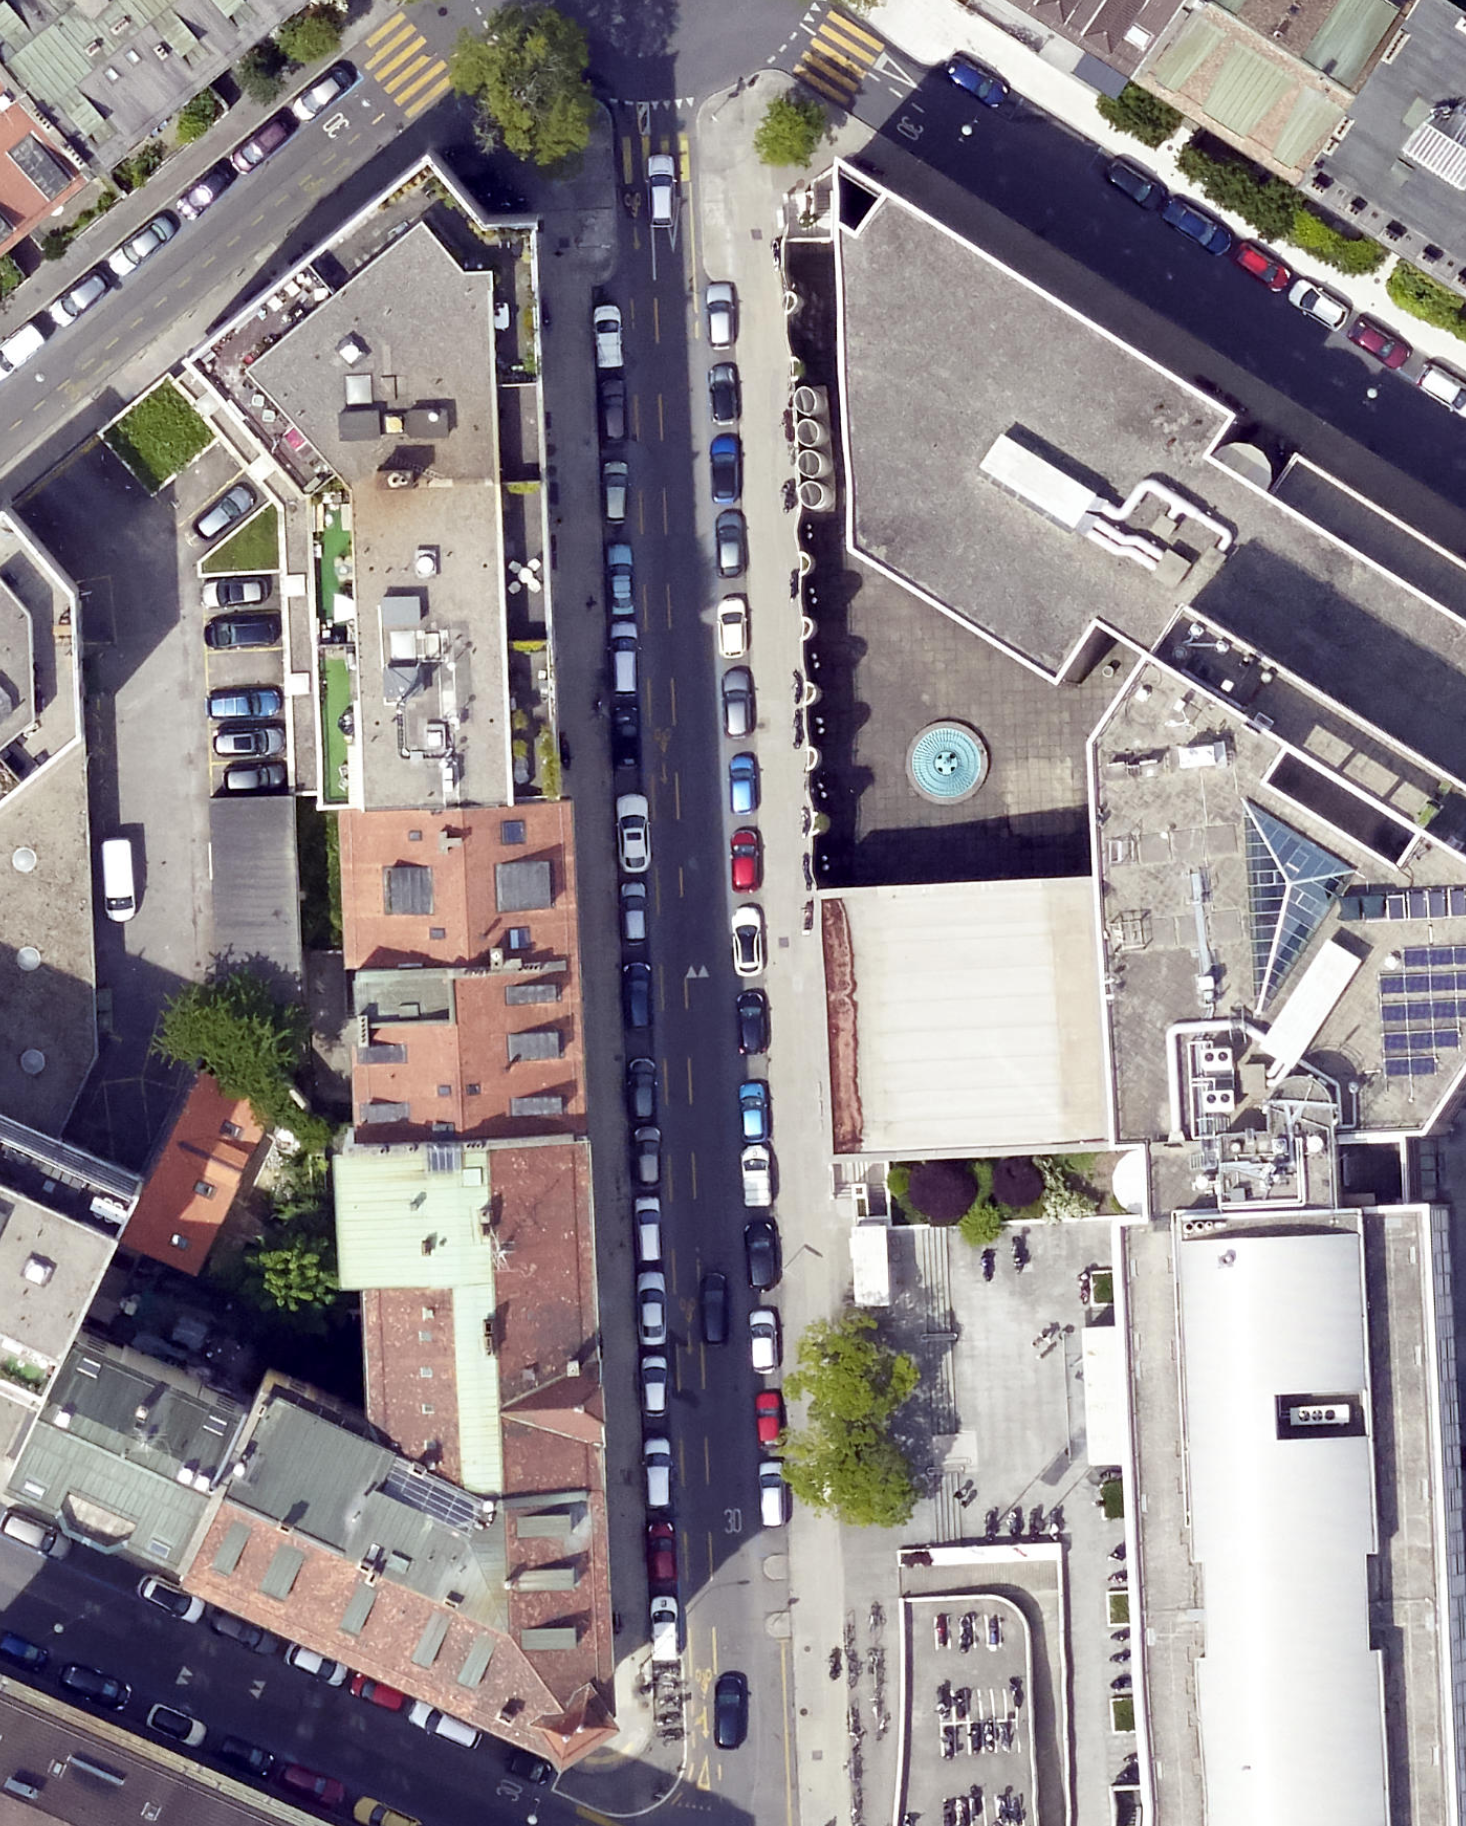
\includegraphics[width=1\linewidth]{02-main//figures/ch3_dataset_methodo_01_orthophoto_2019.png}
    \caption{Orthophotos}
    \label{fig:ch3_dataset_methodo_01_orthophoto_2019}
\end{figure}

\subsubsection{Données vectorielles}
Les données vectorielles choisies sont régulièrement mises à jour. Elles sont au format GPKG \cite{noauthor_ogc_nodate}, ce format est assez commun dans le monde de la géomatique. La sous-section \ref{subsec:annexe_donnees_vectorielles} permet d'avoir un aperçu de ce que sont les données vectorielles.
\paragraph{Bâtiments hors-sol}
La couche vectorielle ``CAD\_BATIMENTS\_HORSOL'' \cite{sitg_batiments_nodate} recense tous les bâtiments du Canton de Genève qui sont bien ancrés au sol. Cette couche n'inclus pas les bâtiments qui sont sous-terrains. La Figure \ref{fig:ch3_dataset_methodo_02_batiment_horsol} permet d'observer ces polygones qui représentent les bâtiments en jaune.

Cette couche vectorielle est enrichie de données tabulaires associées à chacun des polygones. Les données utilisées sont l'``\gls{egid}'' et ``NOMEN\_CLASSE''. L'\gls{egid} est un identifiant unique pour tous les bâtiments en Suisse. ``NOMEN\_CLASSE'' identifie l'usage du bâtiment et va permettre de définir une classe \gls{sia}.

\begin{figure}[H]
    \centering
    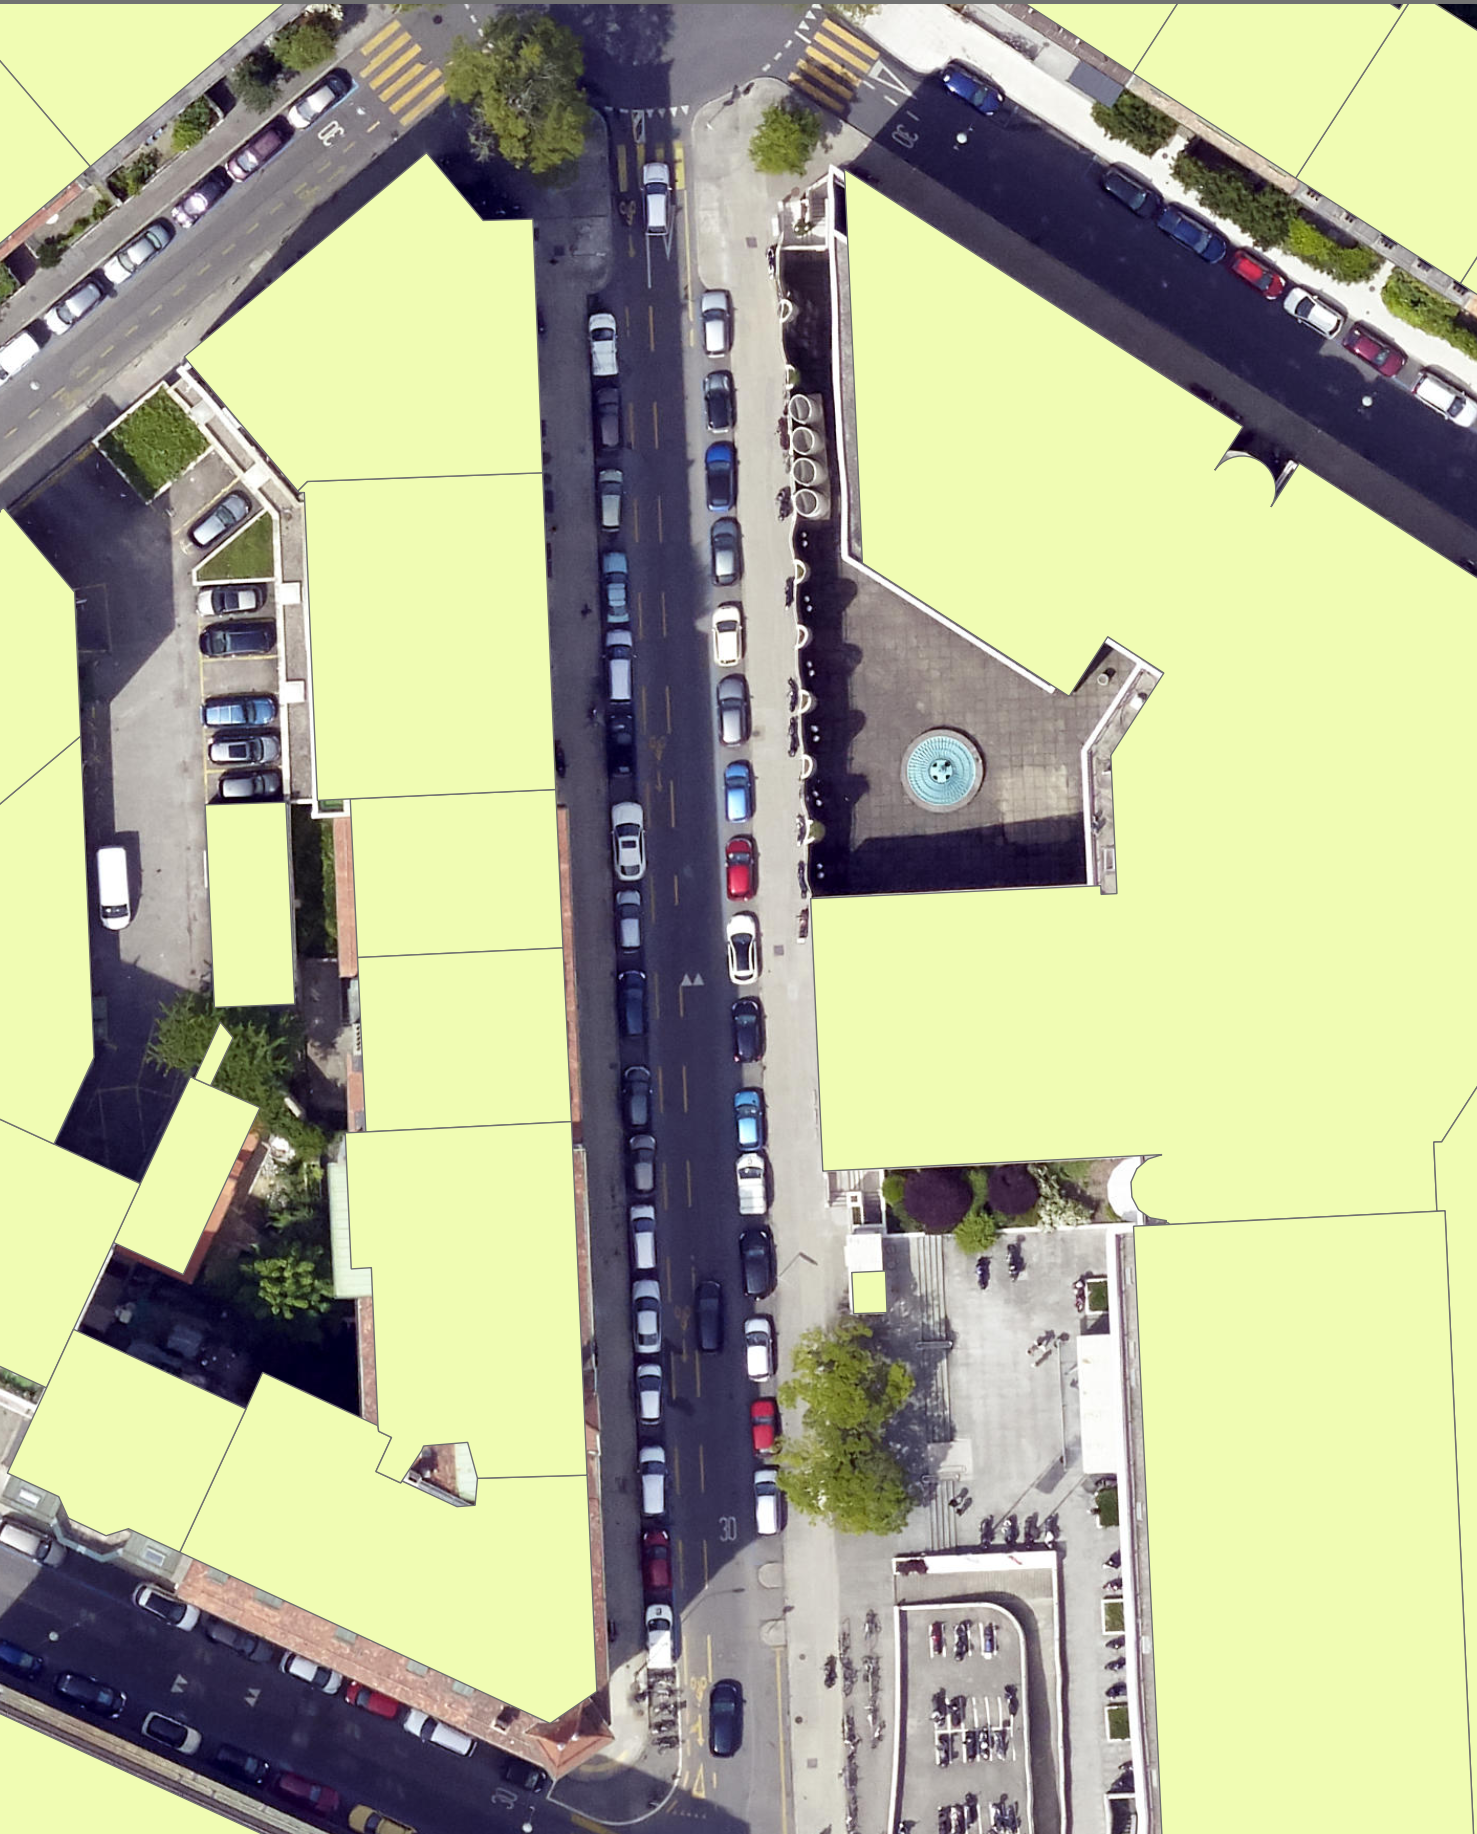
\includegraphics[width=1\linewidth]{02-main//figures/ch3_dataset_methodo_02_batiment_horsol.png}
    \caption{Couche vectorielle bâtiments hors-sol}
    \label{fig:ch3_dataset_methodo_02_batiment_horsol}
\end{figure}


\newpage
\paragraph{Toits des bâtiments}
La couche vectorielle ``CAD\_BATIMENTS\_HORSOL'' \cite{sitg_toits_nodate} regroupe toutes les toitures des bâtiments hors-sol du Canton de Genève (Figure \ref{fig:ch3_dataset_methodo_03_batiment_horsol_toiture}). Un \gls{egid} est associé à chacun des polygones des toitures.

\begin{figure}[H]
    \centering
    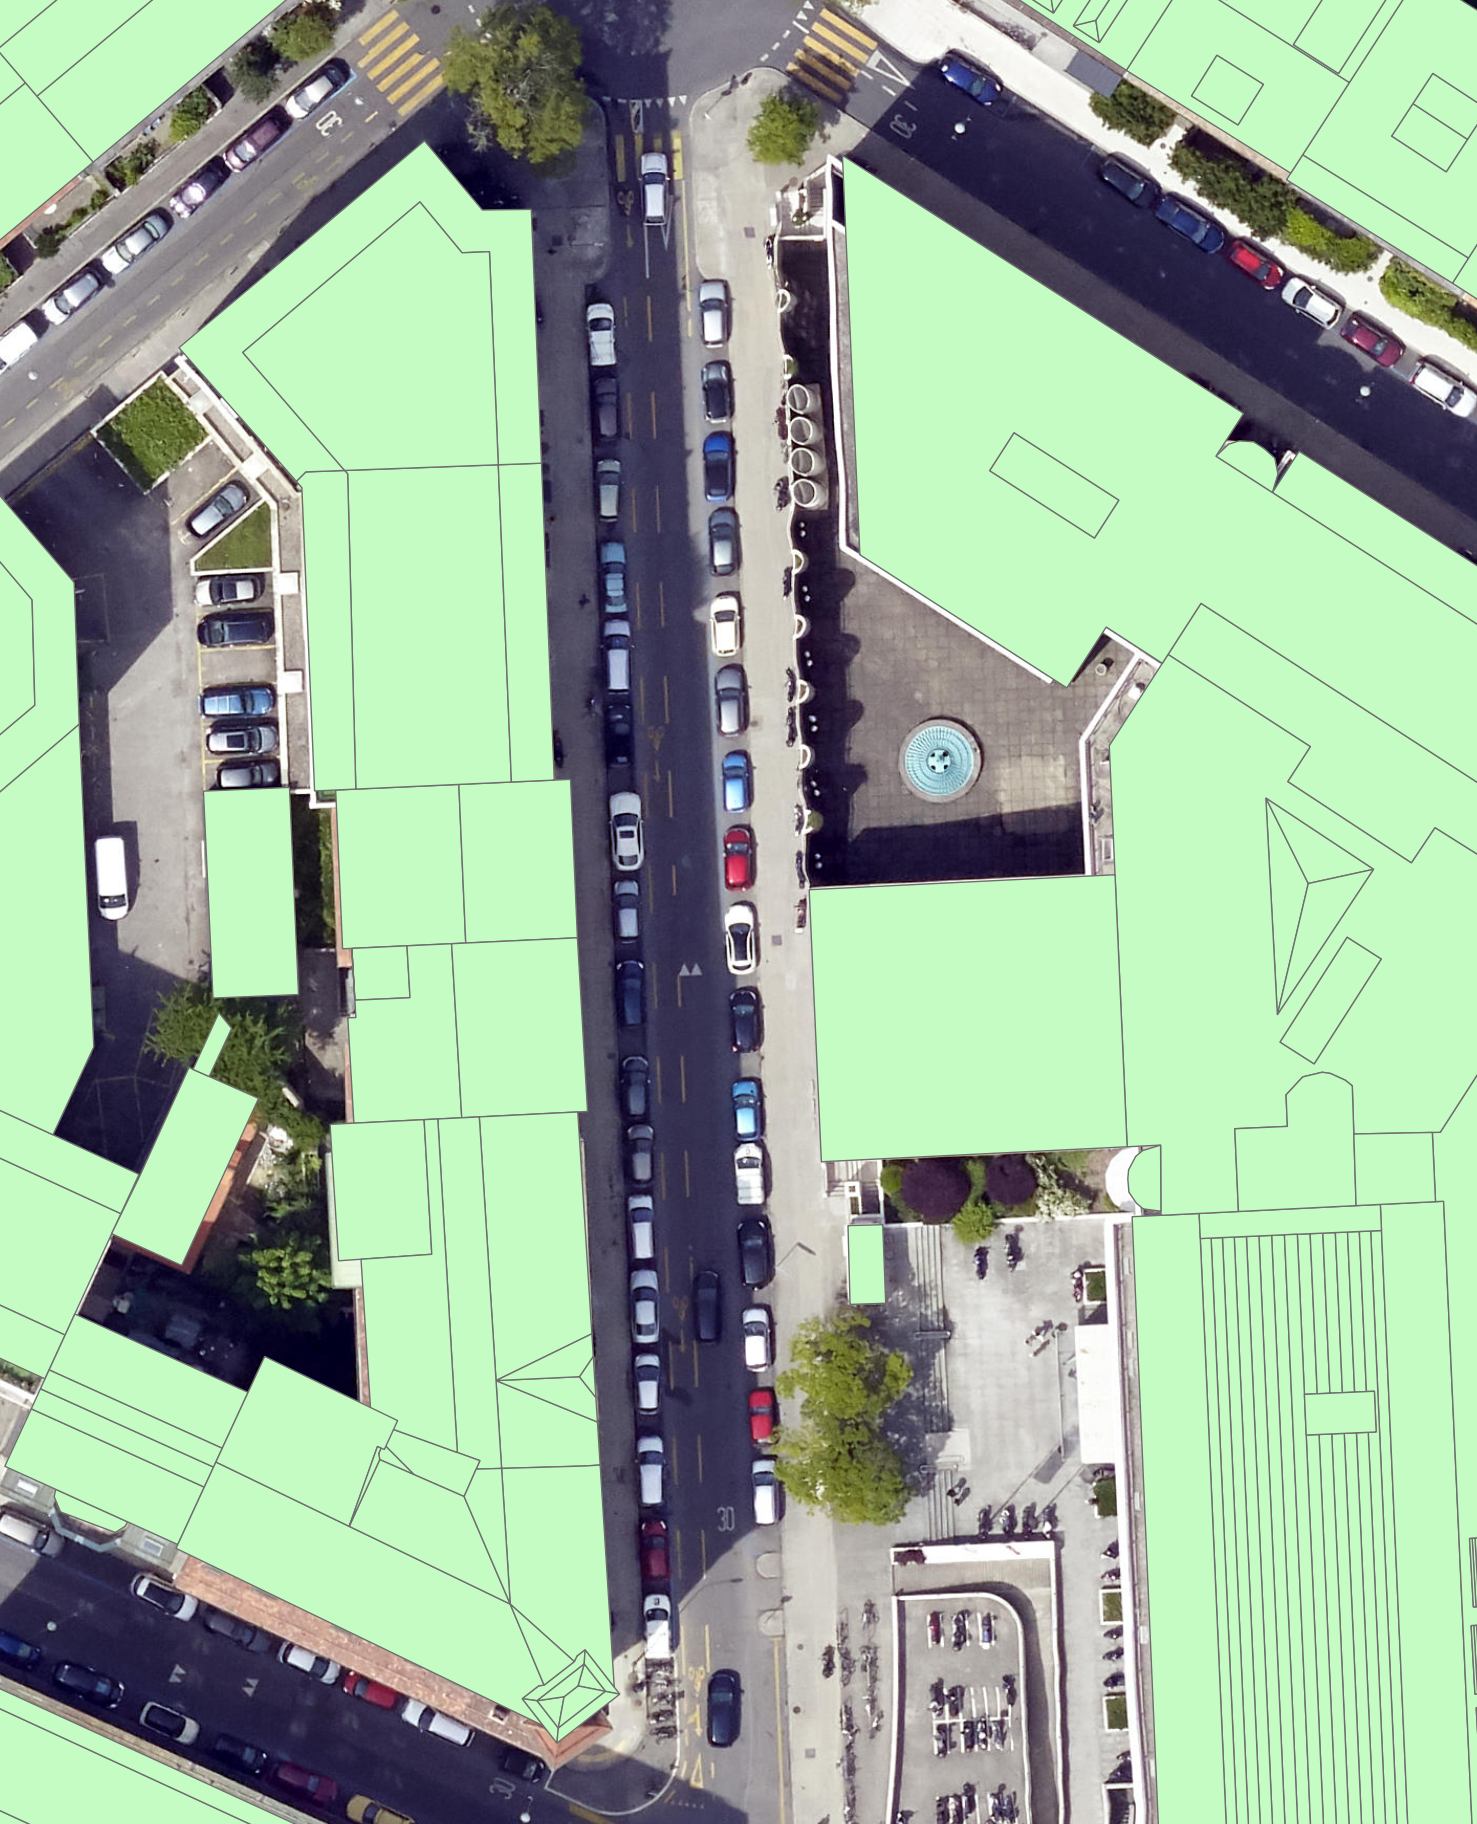
\includegraphics[width=1\linewidth]{02-main//figures/ch3_dataset_methodo_03_batiment_horsol_toiture.png}
    \caption{Couche vectorielle toits des bâtiments}
    \label{fig:ch3_dataset_methodo_03_batiment_horsol_toiture}
\end{figure}

\newpage
\paragraph{Superstructures des toits des bâtiments}
La couche vectorielle ``CAD\_BATIMENT\_HORSOL\_TOIT\_SP'' \cite{sitg_toits_nodate} recense partiellement les superstructures de plus de 9 \si{\unit{\square\meter}} présentes sur les les toitures des bâtiments hors-sol du Canton de Genève (Figure \ref{fig:ch3_dataset_methodo_04_batiment_horsol_toiture_sp}). Un \gls{egid} est associé à chacun des polygones des superstructures.

\begin{figure}[H]
    \centering
    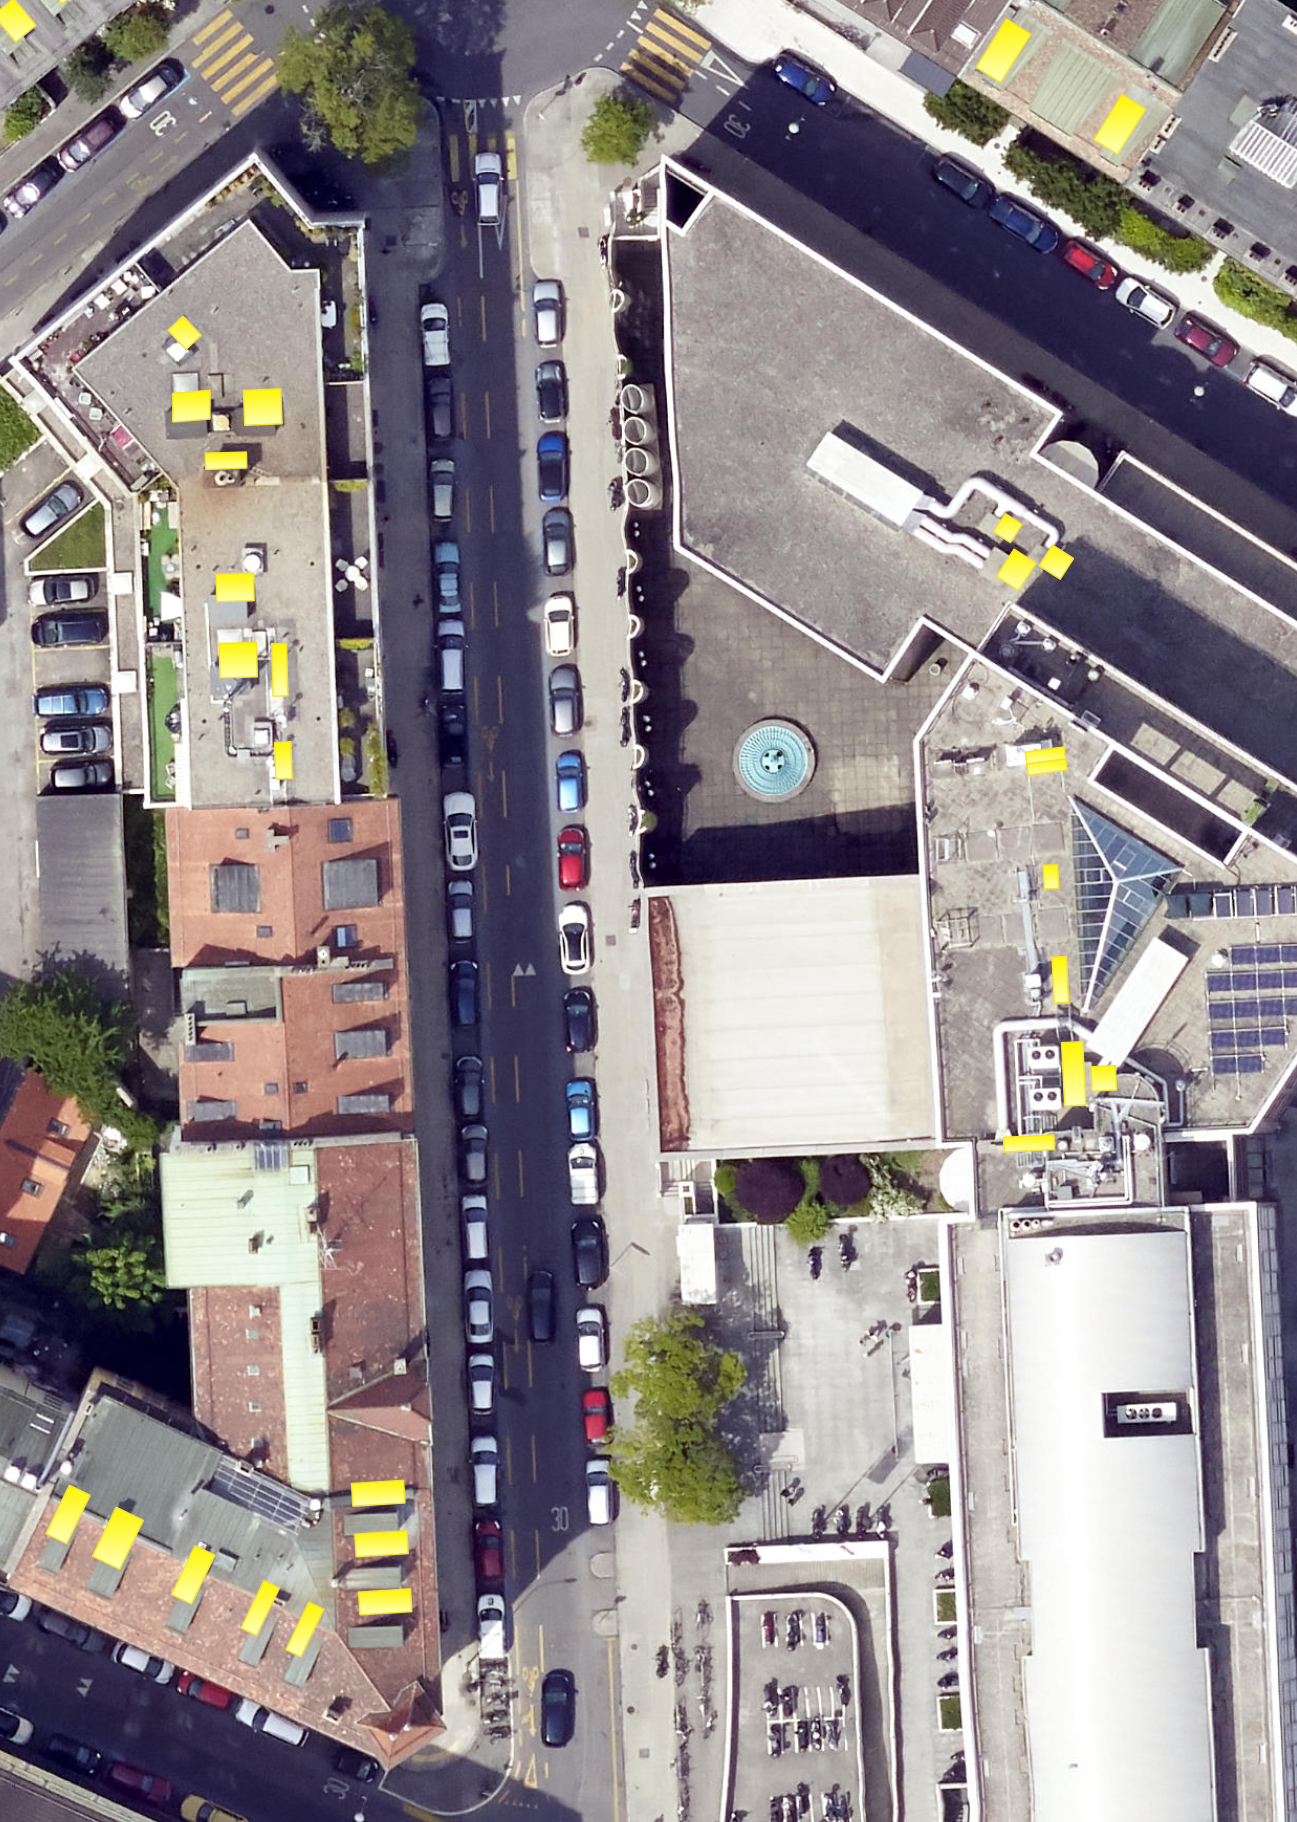
\includegraphics[width=1\linewidth]{02-main//figures/ch3_dataset_methodo_04_batiment_horsol_toiture_sp.png}
    \caption{Couche vectorielle superstructures des toits des bâtiments}
    \label{fig:ch3_dataset_methodo_04_batiment_horsol_toiture_sp}
\end{figure}











\todo[inline]{Ajouter ici le lien correct à l'annexe des données vectorielles}







% -----------------------------------------------------------------------------
% -----------------------------------------------------------------------------
\newpage
\section{Autres pistes explorées}
\label{sec:pistes_explorees}
Plusieurs autres approches ont été explorées, le but initial étant d'éviter de devoir créer un dataset. La génération d'un dataset pour une tâche tel que la segmentation sémantique est assez chronophage et laborieux. La première approche est d'essayer de classifier les données géomatiques, la deuxième approche implique l'utilisation de segment-anything-model.

\subsection{Classification}
La classification des toitures est une approche naïve pour déterminer quelles toitures sont disponibles en utilisant les couches des toitures et superstructures de \acrshort{sitg}.

\subsubsection{Méthodologie}
La Figure \ref{fig:ch3_piste_exploree_classification_01_workflow} résume les principales étapes. 

\begin{figure}[H]
    \centering
    \makebox[\textwidth]{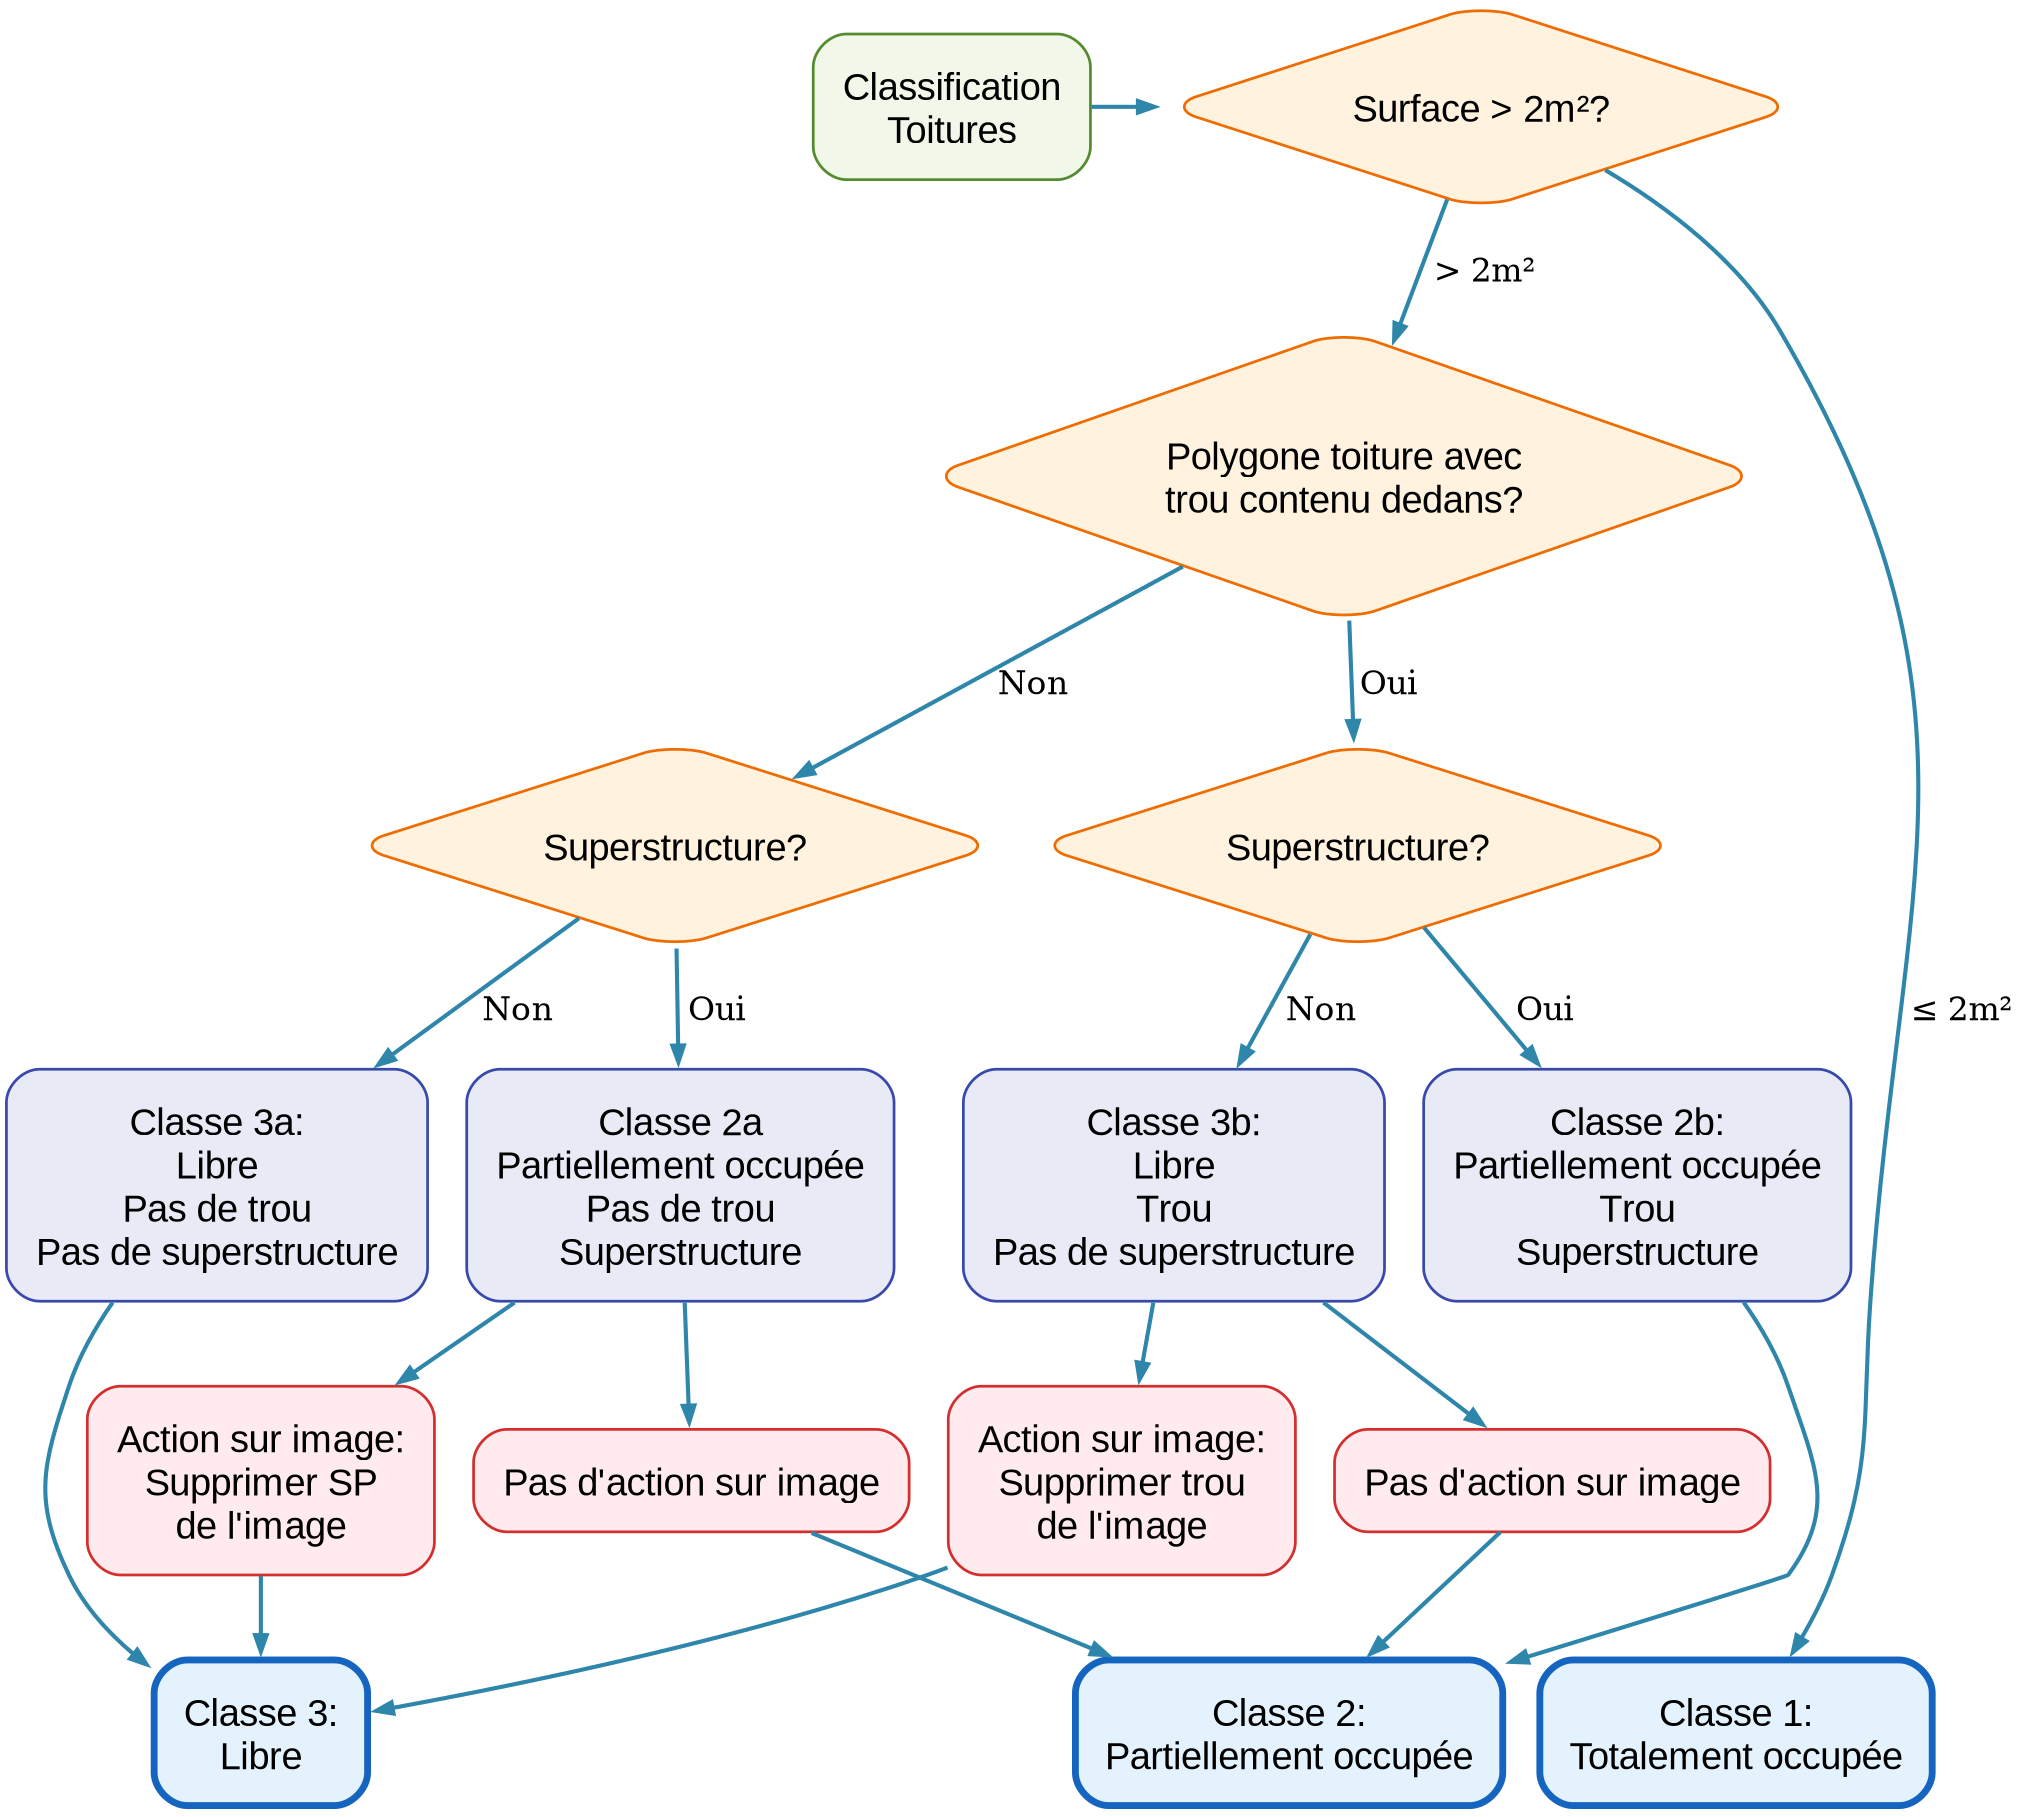
\includegraphics[width=1.3\linewidth]{02-main//figures/ch3_piste_exploree_classification_01_workflow.png}}
    \caption{Schéma classification des toitures}
    \label{fig:ch3_piste_exploree_classification_01_workflow}
\end{figure}

L'objectif est de créer 3 classes en utilisant la couche des toitures et celle des superstructures:
\begin{itemize}
    \item Classe 1: Toiture totalement occupée
    \item Classe 2: Toiture partiellement occupée
    \item Classe 3: Toiture libre
\end{itemize}
Premièrement, les toitures de moins de 2 \si{\unit{\square\meter}} sont éliminées car jugées trop petites.

L'étape suivante (Figure \ref{fig:piste_exploree_classification_image_exemple}) est de déterminer si la toiture est un polygone complètement fermé ou s'il y a un autre polygone à l'intérieur. La Figure \ref{fig:ch3_piste_exploree_classification_02_image_originale} représente une image d'exemple pour illustrer cette étape, la toiture est un toit à deux pans inclinés avec des lucarnes. La Figure \ref{fig:ch3_piste_exploree_classification_03_couche_toiture} superpose la couche des toitures sur la Figure \ref{fig:ch3_piste_exploree_classification_02_image_originale}, on observe que la couche des toitures a bien un polygone assigné à chacune des lucarnes. La Figure \ref{fig:ch3_piste_exploree_classification_04_image_resultante} représente le résultat pour la partie nord de la toiture, la partie intérieur (lucarne) a été éliminée et tout ce qui est hors polygone a été enlevé.

A continuation, il faut vérifier la présence d'une superstructure (couche superstructure) sur la toiture. Dans le cas de la Figure \ref{fig:piste_exploree_classification_image_exemple}, il n'y a pas de superstructure dans la toiture.

Les deux étapes précédentes vont déterminer l'action à réaliser sur l'image, ainsi que sa classification. Si l'on reprend le schéma de la Figure \ref{fig:ch3_piste_exploree_classification_01_workflow} pour l'exemple étape par étape:
\begin{enumerate}
    \item Surface > 2 \si{\unit{\square\meter}} : Oui
    \item Polygone totalement inclus à l'intérieur de celui de la toiture : Oui
    \item Superstructure sur la toiture : Non
    \item Classe 3b: Supprimer "trou" de l'image
    \item Toiture finalement classée comme "libre"
\end{enumerate}

\begin{figure}[H]
    \centering
    
    % Première ligne
    \begin{subfigure}[b]{0.475\textwidth}
        \centering
        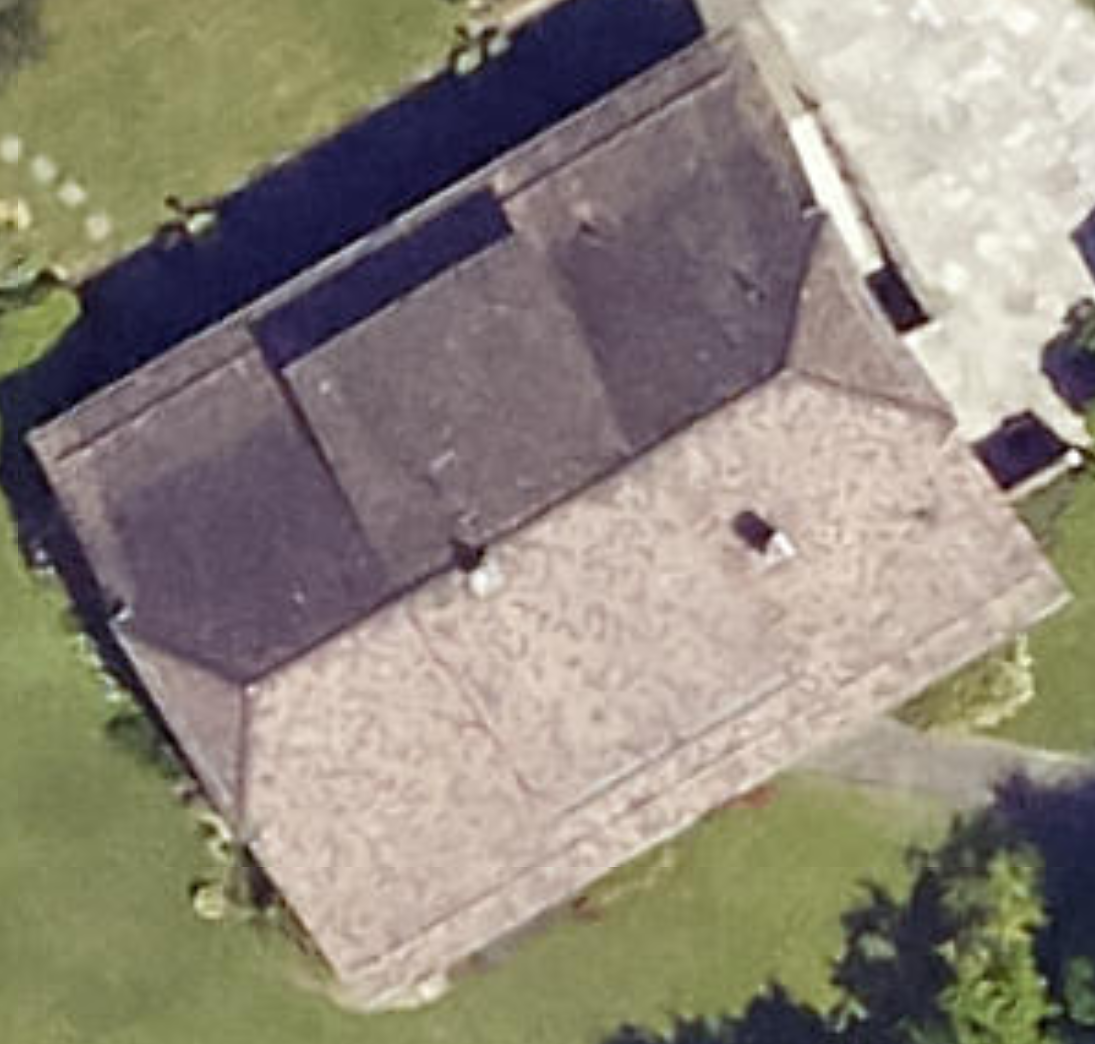
\includegraphics[width=\textwidth]{02-main/figures/ch3_piste_exploree_classification_02_image_originale.png}
        \caption{Image d'exemple}
        \label{fig:ch3_piste_exploree_classification_02_image_originale}
    \end{subfigure}
    \hfill
    \begin{subfigure}[b]{0.48\textwidth}
        \centering
        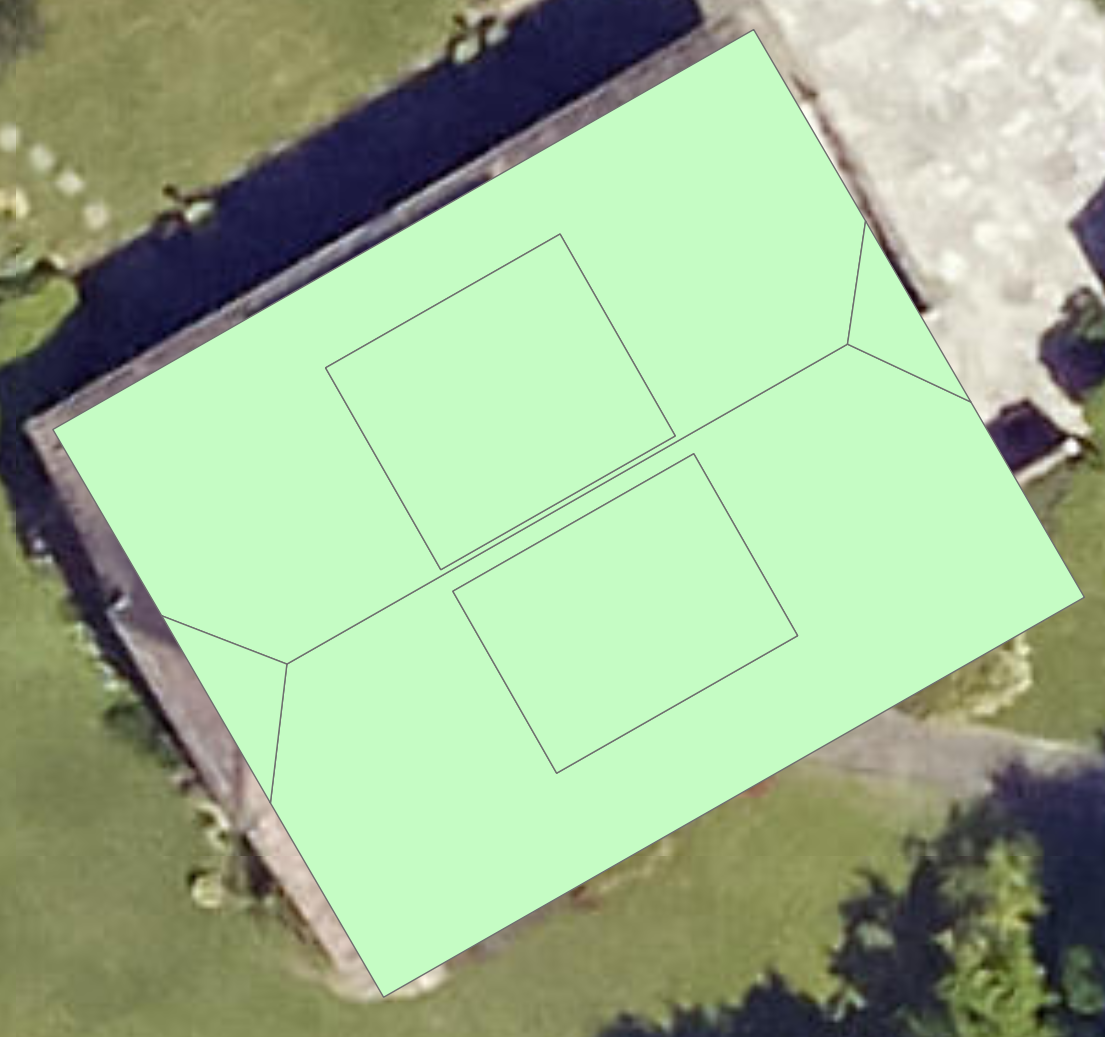
\includegraphics[width=\textwidth]{02-main/figures/ch3_piste_exploree_classification_03_couche_toiture.png}
        \caption{Couche toiture superposée}
        \label{fig:ch3_piste_exploree_classification_03_couche_toiture}
    \end{subfigure}
    
    \vspace{0.35cm} % Espace entre les lignes
    
    % Deuxième ligne
    \begin{subfigure}[b]{0.48\textwidth}
        \centering
        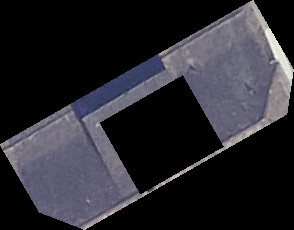
\includegraphics[width=\textwidth]{02-main/figures/ch3_piste_exploree_classification_04_image_resultante.png}
        \caption{Résultat final}
        \label{fig:ch3_piste_exploree_classification_04_image_resultante}
    \end{subfigure}

    \caption{Exemple de toiture avec un "trou" et sans superstructure}
    \label{fig:piste_exploree_classification_image_exemple}
\end{figure}

\subsubsection{Résultats}

La Figure \ref{fig:ch3_piste_exploree_classification_05_classification_simplified} représente la classification intermédiaire selon la présence d'un polygone à l'intérieur de la toiture et de la présence de superstructure (voir Figure \ref{fig:ch3_piste_exploree_classification_01_workflow}). La grande majorité des toitures sont classées comme "3a", c'est à dire des toitures qui n'ont pas de superstructure ni d'autre polygone à l'intérieur. Ce sont des toitures à priori libres.

La Figure \ref{fig:ch3_piste_exploree_classification_06_classification_finale} montre la classification finale en 3 classes. Les résultats indiquent que quasiment toutes les toitures sont libres, ce qui est loin d'être le cas. Le problème est la couche des superstructures, celle-ci n'est pas complète et pas tous les éléments en dessous de 9 \si{\unit{\square\meter}} sont représentés. La classification ne tient pas en compte de la réalité terrain et sa précision et pertinence va dépendre de la qualité des données géomatiques utilisées.

\begin{figure}[H]
    \centering
    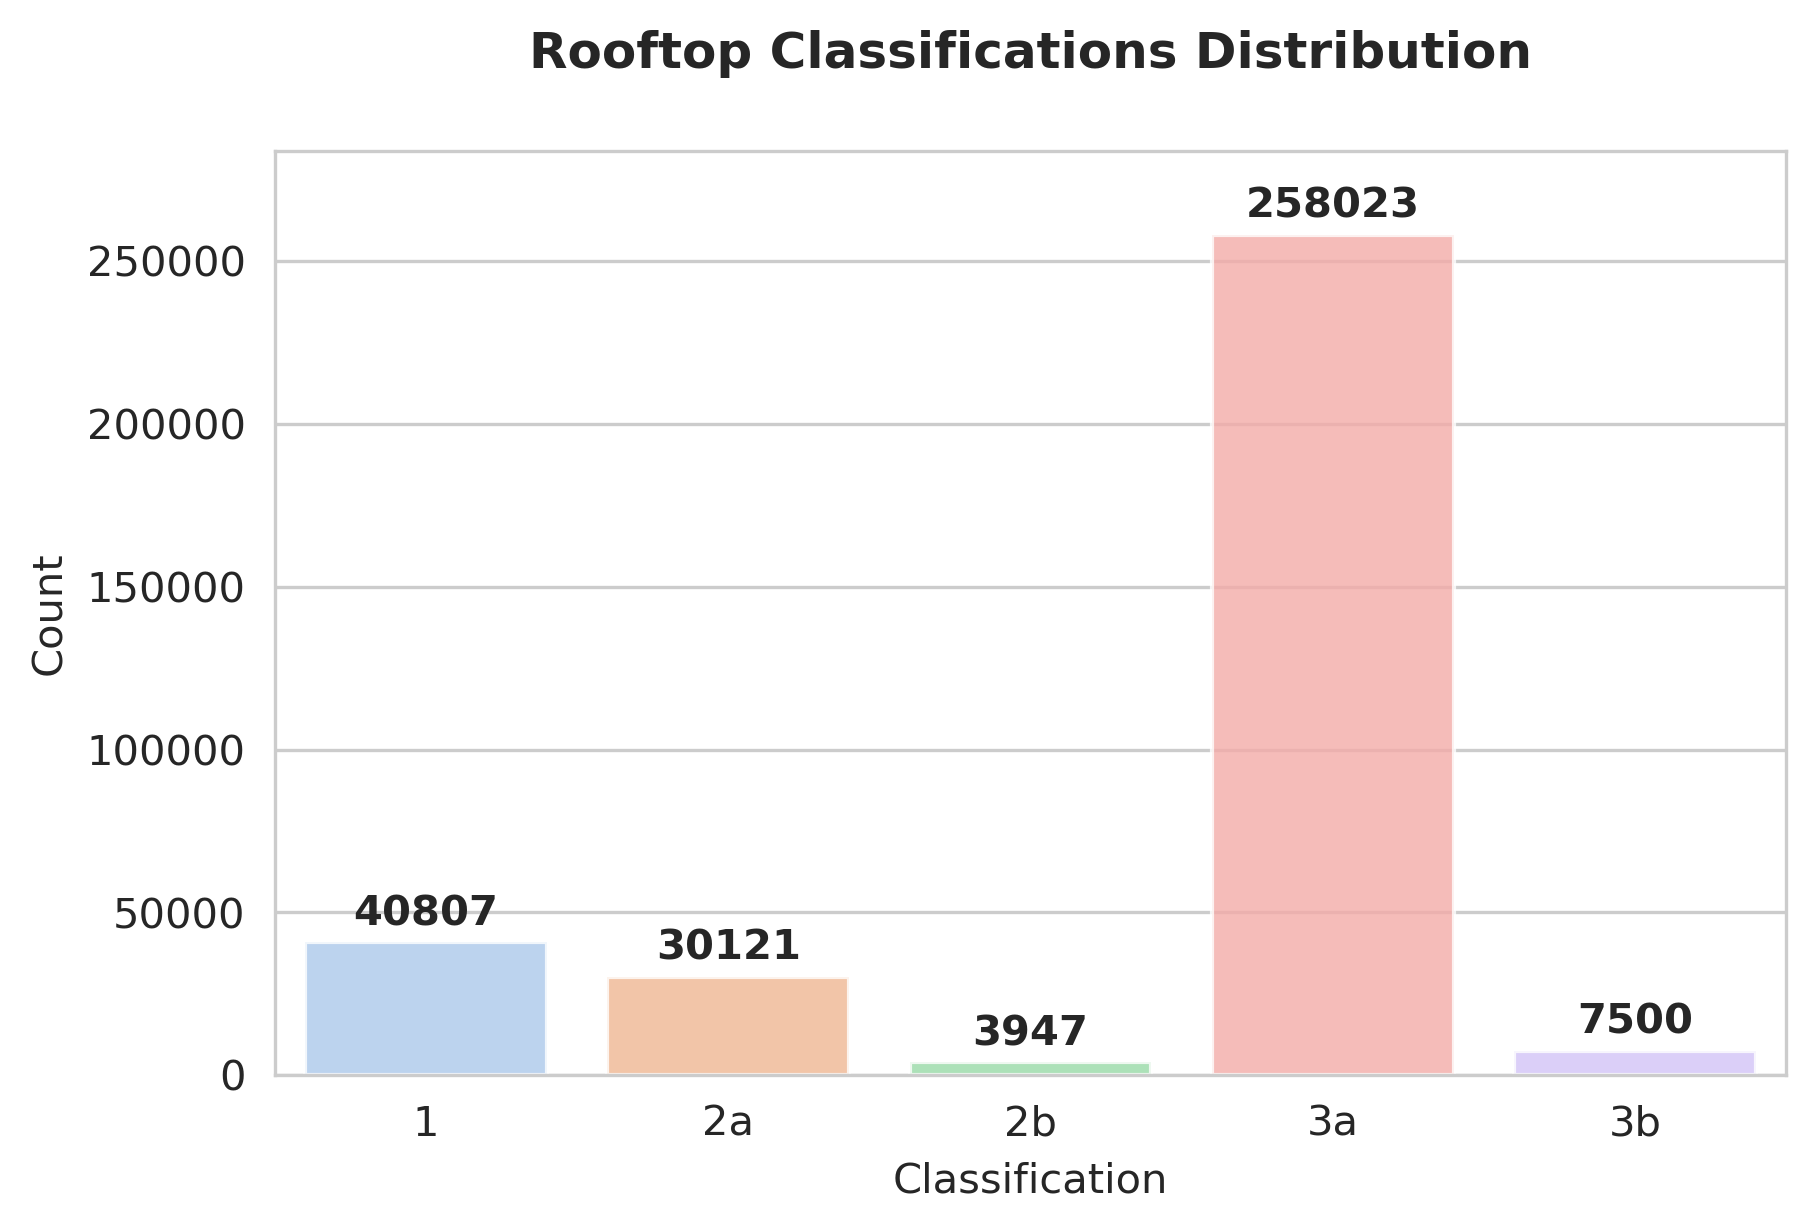
\includegraphics[width=1\linewidth]{02-main//figures/ch3_piste_exploree_classification_05_classification_intermediaire.png}
    \caption{Classification intermédiaire}
    \label{fig:ch3_piste_exploree_classification_05_classification_simplified}
\end{figure}

\begin{figure}[H]
    \centering
    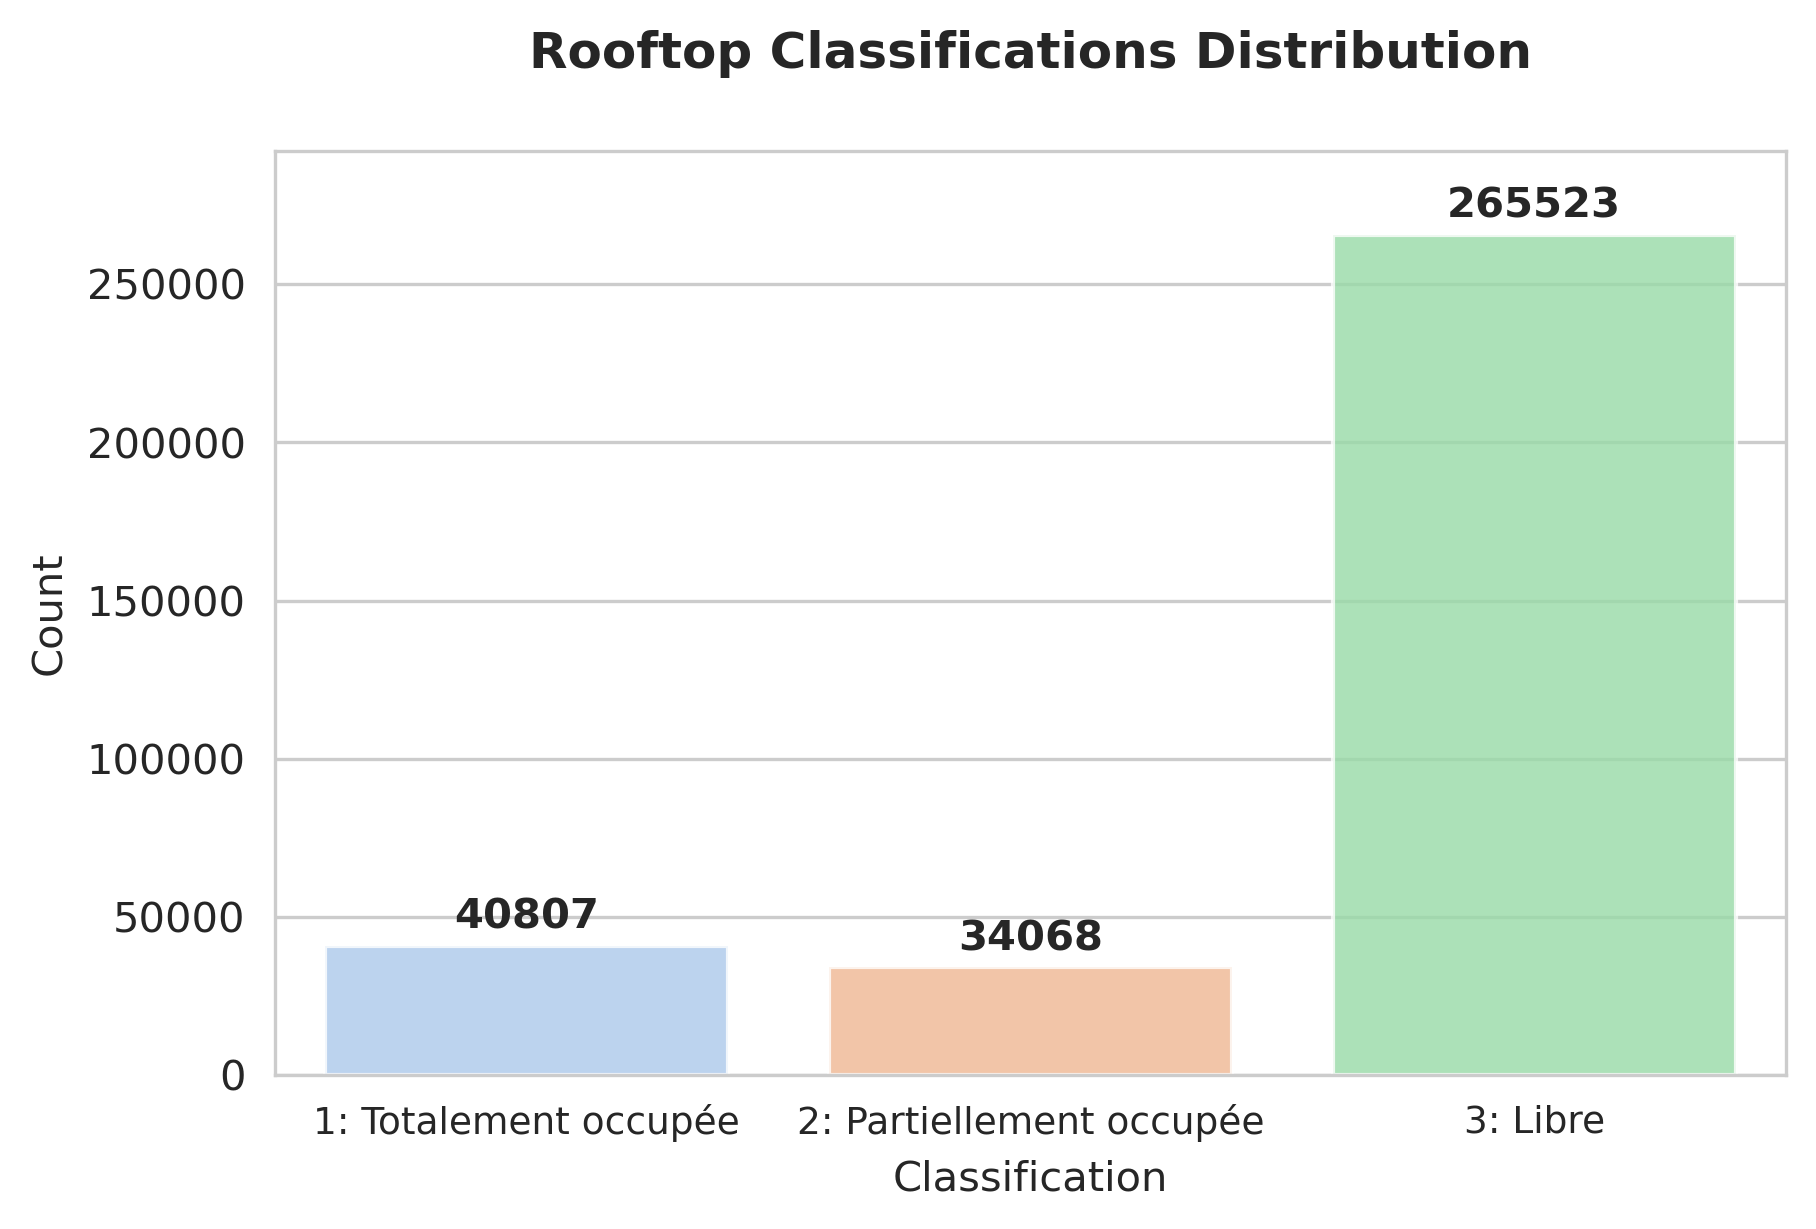
\includegraphics[width=1\linewidth]{02-main//figures/ch3_piste_exploree_classification_06_classification_finale.png}
    \caption{Classification finale}
    \label{fig:ch3_piste_exploree_classification_06_classification_finale}
\end{figure}

La Figure \ref{fig:piste_exploree_classification_resultats_explications} représente un exemple de la problématique, les superstructures présentes sur le toit (Figure \ref{fig:ch3_piste_exploree_classification_10_resultats_image_sp}) ne sont pas toutes représentées (Figure \ref{fig:ch3_piste_exploree_classification_07_resultats_image_exemple}). La couche des toitures (Figure \ref{fig:ch3_piste_exploree_classification_08_resultats_image_toiture}) inclus aussi des balcons et terrasses, ce qui complique significativement la tâche de classification. Il n'y a pas le découpage pour cette toiture (similaire Figure \ref{fig:ch3_piste_exploree_classification_04_image_resultante}), car il y a un bug dans le script qui classifie et découpe les toitures. Finalement, il y a aussi des problèmes d’alignement entre les orthophotos et les superstructures qui rendent peu fiables les découpes nécessaires pour enlever les superstructures des toitures dans la dernière phase de la classification.

\begin{figure}[H]
    \centering
    
    % Première ligne
    \begin{subfigure}[b]{0.475\textwidth}
        \centering
        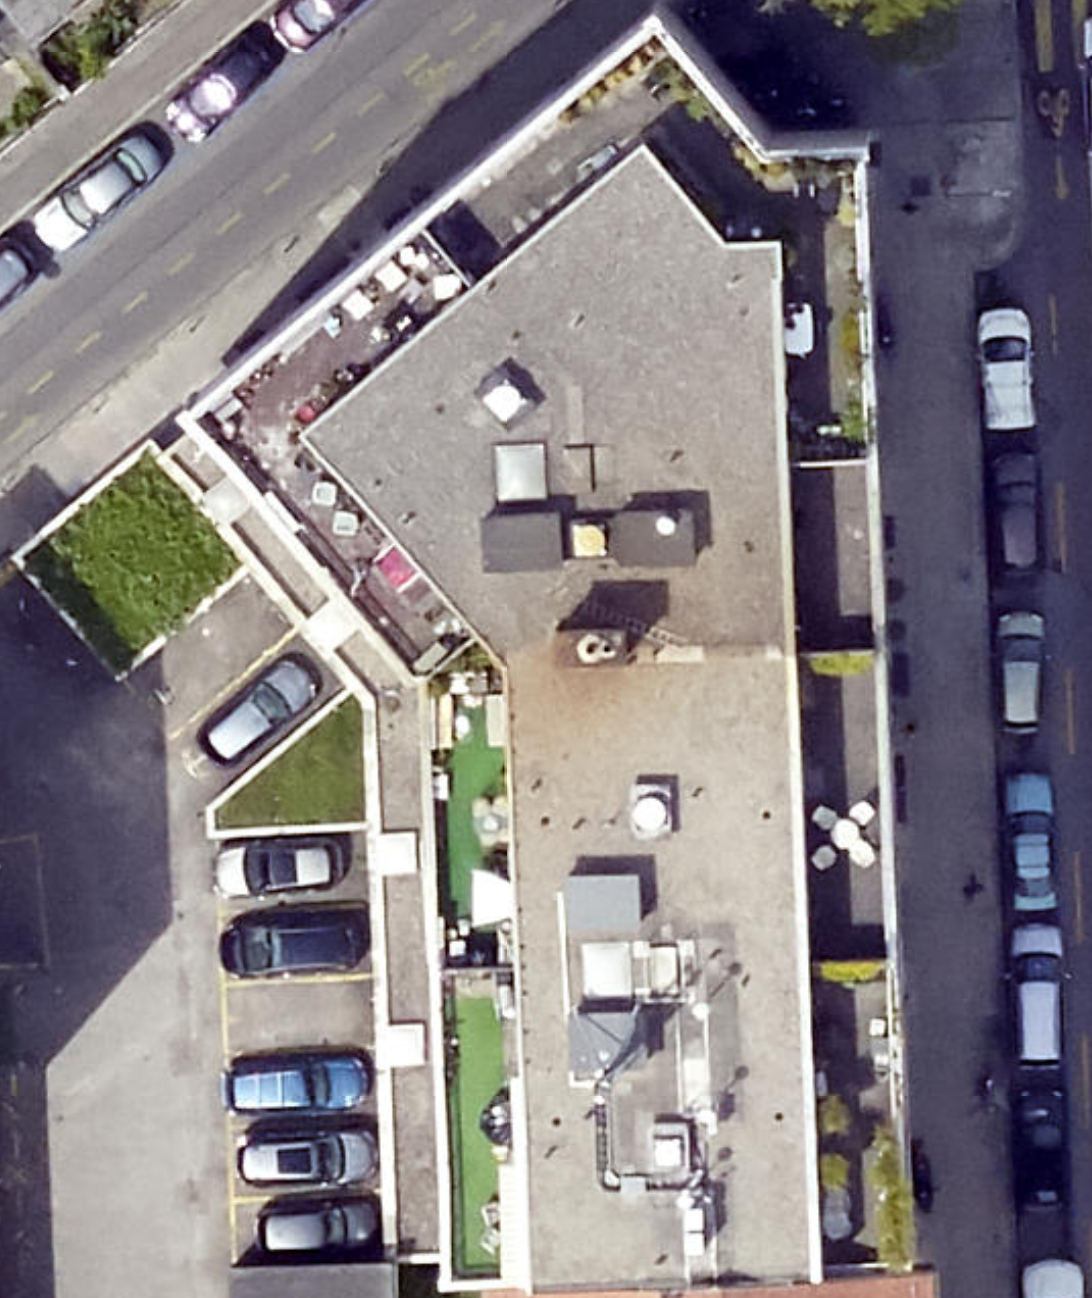
\includegraphics[width=\textwidth]{02-main/figures/ch3_piste_exploree_classification_07_resultats_image_exemple.png}
        \caption{Image d'exemple}
        \label{fig:ch3_piste_exploree_classification_07_resultats_image_exemple}
    \end{subfigure}
    \hfill
    \begin{subfigure}[b]{0.48\textwidth}
        \centering
        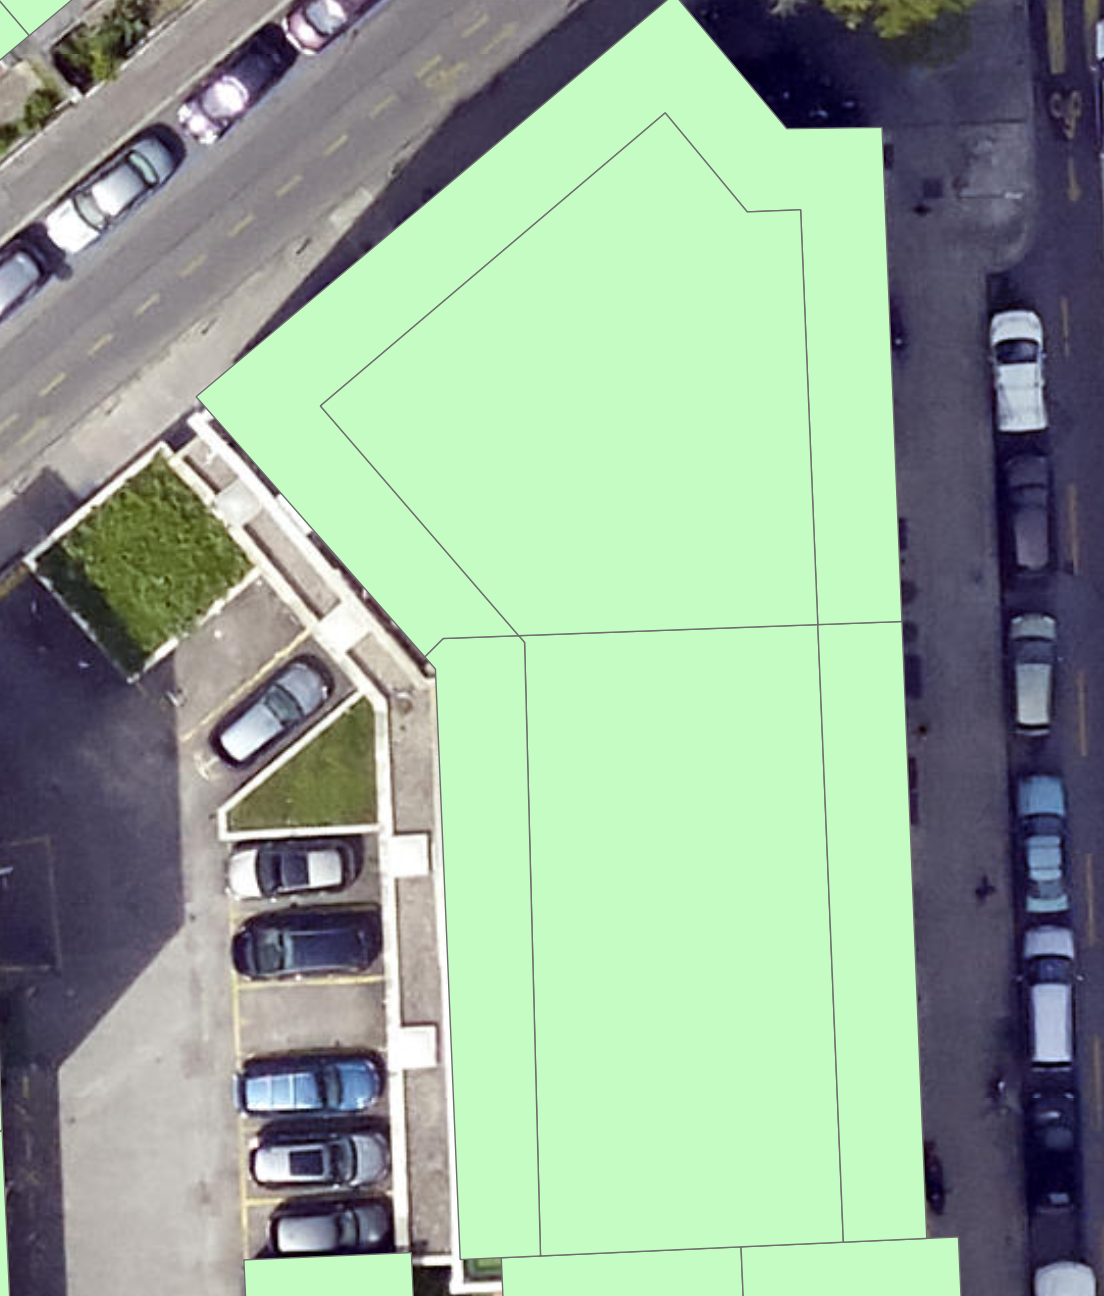
\includegraphics[width=\textwidth]{02-main/figures/ch3_piste_exploree_classification_08_resultats_image_toiture.png}
        \caption{Couche des toitures}
        \label{fig:ch3_piste_exploree_classification_08_resultats_image_toiture}
    \end{subfigure}
    
    \vspace{0.35cm} % Espace entre les lignes
    
    % Deuxième ligne
    \begin{subfigure}[b]{0.48\textwidth}
        \centering
        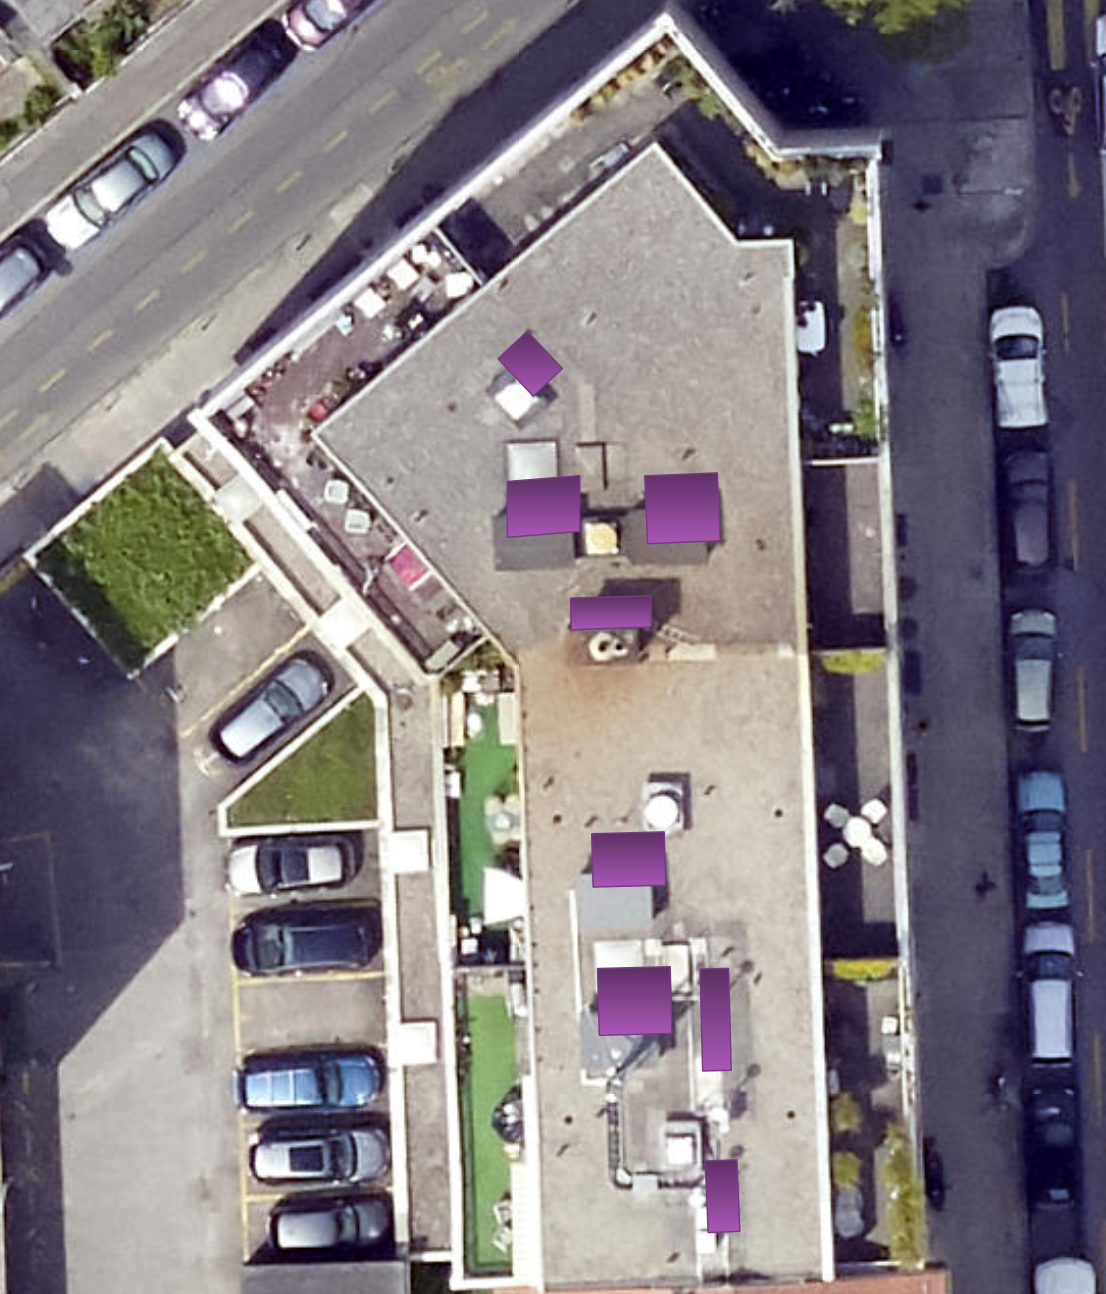
\includegraphics[width=\textwidth]{02-main/figures/ch3_piste_exploree_classification_10_resultats_image_sp.png}
        \caption{Couche des superstructures}
        \label{fig:ch3_piste_exploree_classification_10_resultats_image_sp}
    \end{subfigure}
    \hfill
    \begin{subfigure}[b]{0.475\textwidth}
        \centering
        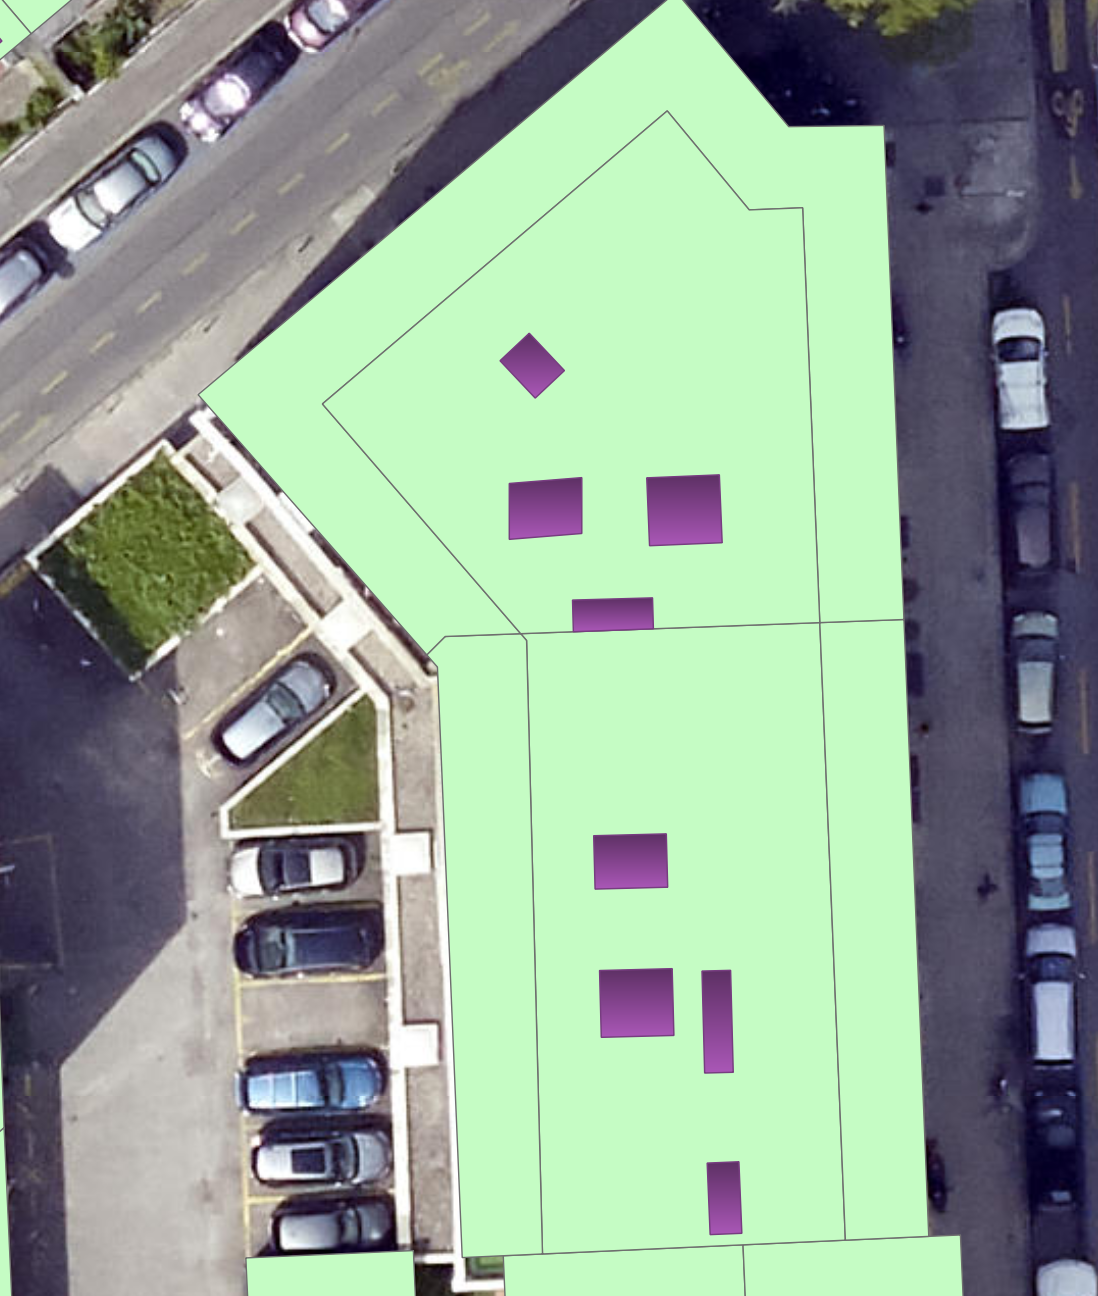
\includegraphics[width=\textwidth]{02-main/figures/ch3_piste_exploree_classification_09_resultats_image__toiture_sp.png}
        \caption{Couche des toitures et superstructures}
        \label{fig:ch3_piste_exploree_classification_09_resultats_image__toiture_sp}
    \end{subfigure}

    \caption{Exemple de toiture problématique pour la classification}
    \label{fig:piste_exploree_classification_resultats_explications}
\end{figure}

Pour conclure, les différents problèmes rencontrés et le manque de fiabilité du résultat final ont fait que la piste de la classification n'a pas été retenue.


\newpage
\subsection{SAM}
Une autre piste explorée est l'utilisation de segment-anything-model (SAM). Cet algorithme a l'avantage de permettre une segmentation efficace sur des images sur lesquels SAM n'a pas spécifiquement été entraîné. \acrshort{stdl} avait déjà exploré cette piste (section \ref{subsec:stdl_analyse}) avec quelques différences entre les méthodologies utilisée.

\subsubsection{Méthodologie}
La Figure \ref{fig:essai_algo_sam} résume les différentes étapes:
\begin{enumerate}
    \item Mettre en noir tout ce qui est hors toiture (Figure \ref{fig:ch3_essai_sam_01_image_original})
    \item Détermination zone d'intêret (Figure \ref{fig:ch3_essai_sam_02_ROI})
    \item SAM va segmenter toute l'image (Figure \ref{fig:ch3_essai_sam_03_200_masks})
    \item Filtrer les masques (polygones segmentés) (Figure \ref{fig:ch3_essai_sam_04_194_filtered_masks})
    \item Visualisation des masques filtrés avec des couleurs plus vives pour vérification visuelle (Figure \ref{fig:ch3_essai_sam_05_filtered_masks_overlay})
    \item Détermination de l'espace libre (Figure \ref{fig:ch3_essai_sam_06_une_zone_libre})
\end{enumerate}

La première étape (Figure \ref{fig:ch3_essai_sam_01_image_original}) est de fusionner tous les polygones qui délimitent la toiture. Ce grand polygone de toiture va permettre de centrer l'attention de SAM sur la toiture, les zones hors toitures peuvent être considérées comme du bruit et mises en noir. Un avantage notable de cette démarche est d'éviter du temps de calcul à SAM.

La deuxième étape (Figure \ref{fig:ch3_essai_sam_02_ROI}) est de déterminer la zone d'intérêt (ROI). Cette étape utilise la librairie python pillow et permet de mettre en évidence les zones sombres à l'intérieur de la toiture.

La troisième étape (Figure \ref{fig:ch3_essai_sam_03_200_masks}) utilise l'algorithme SAM pour réaliser la segmentation complète de l'image de la Figure \ref{fig:ch3_essai_sam_01_image_original}. Dans ce cas, un total de 200 masques sont segmentés. Le temps de calcul est de 7 minutes pour une image de toiture. SAM dispose de plusieurs paramètres qui peuvent augmenter significativement le temps de calcul; SAM peut par exemple diviser l'image en plusieurs parties pour améliorer la segmentation, plus cette partition est fine, meilleurs seront les résultats. La documentation de SAM est assez rudimentaire et n'explique pas clairement toutes les options disponibles.

La quatrième étape (Figure \ref{fig:ch3_essai_sam_04_194_filtered_masks}) consiste à filtrer les polygones segmentés selon trois critères principaux :
\begin{itemize}
    \item Recouvrement avec la ROI : les masques doivent avoir un recouvrement supérieur à 50\% avec la zone d'intérêt
    \item Taille minimale : élimination des polygones de moins de 50 pixels (paramètre SAM) et suppression additionnelle des masques avec moins de 100 pixels
    \item Qualité de segmentation : utilisation des seuils SAM avec un IoU prédit > 0.85 et un score de stabilité > 0.85
\end{itemize}
Cette étape réduit le nombre de masques de 200 à 194, éliminant principalement les artefacts de segmentation hors toiture et les zones trop petites.

La cinquième étape (Figure \ref{fig:ch3_essai_sam_05_filtered_masks_overlay}) propose une visualisation colorée des masques filtrés pour faciliter la vérification visuelle des résultats de segmentation.

La sixième étape (Figure \ref{fig:ch3_essai_sam_06_une_zone_libre}) détermine l'espace libre en combinant plusieurs critères :

\begin{itemize}
    \item Critères géométriques:
    \begin{itemize}
        \item Zone tampon de 0.5 m autour des obstacles détectés
        \item Ratio de largeur/hauteur pour éliminer les masques long mais pas suffisament larges pour être intéressants pour la pose de panneaux solaires
        \item Taille du masque minimum de 10 m² par défaut (soit 4000 pixels à 5 cm/pixel)
    \end{itemize}
    \item Critère de luminosité:
        \begin{itemize}
            \item Filtre sur les zone sombres qui ont une luminosité de moins de 60\% de la moyenne globale de l'image
        \end{itemize}
\end{itemize}

\begin{figure}[H]
    \centering
    
    % Première ligne
    \begin{subfigure}[b]{0.48\textwidth}
        \centering
        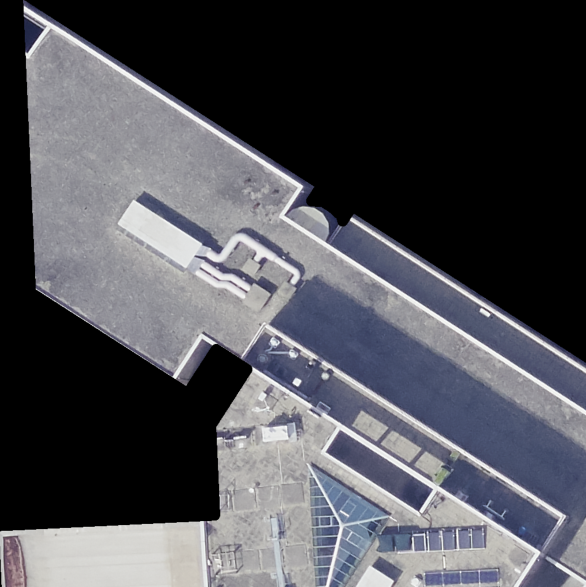
\includegraphics[width=\textwidth]{02-main/figures/ch3_essai_sam_01_image_original.png}
        \caption{Image d'exemple}
        \label{fig:ch3_essai_sam_01_image_original}
    \end{subfigure}
    \hfill
    \begin{subfigure}[b]{0.48\textwidth}
        \centering
        
\includegraphics[width=\textwidth]{02-main/figures/ch3_essai_sam_02_ROI.png}
        \caption{Zone d’intérêt (ROI)}
        \label{fig:ch3_essai_sam_02_ROI}
    \end{subfigure}
    
    \vspace{0.35cm} % Espace entre les lignes
    
    % Deuxième ligne
    \begin{subfigure}[b]{0.48\textwidth}
        \centering
        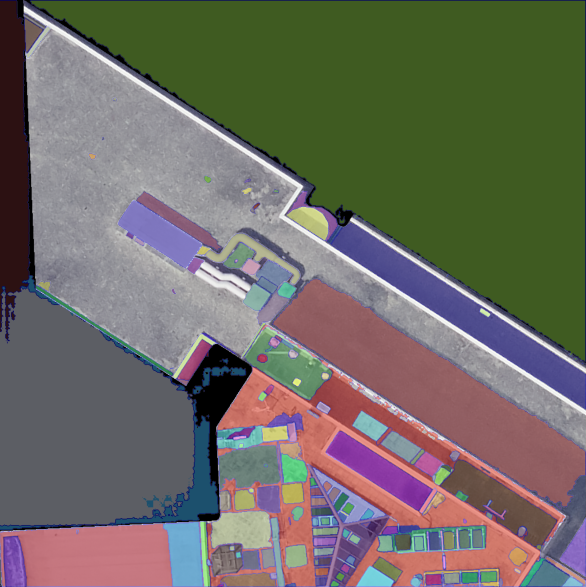
\includegraphics[width=\textwidth]{02-main/figures/ch3_essai_sam_03_200_masks.png}
        \caption{Polygones segmentés (200)}
        \label{fig:ch3_essai_sam_03_200_masks}
    \end{subfigure}
    \hfill
    \begin{subfigure}[b]{0.48\textwidth}
        \centering
        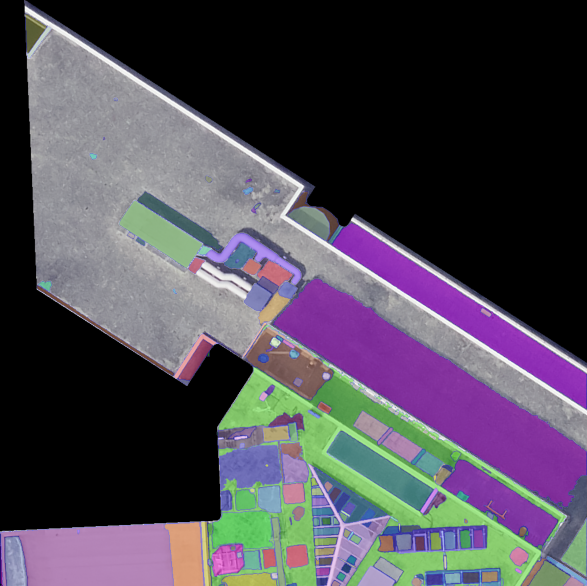
\includegraphics[width=\textwidth]{02-main/figures/ch3_essai_sam_04_194_filtered_masks.png}
        \caption{Polygone segmentés filtrés (194)}
        \label{fig:ch3_essai_sam_04_194_filtered_masks}
    \end{subfigure}

    \vspace{0.35cm} % Espace entre les lignes
    
    % Troisième ligne
    \begin{subfigure}[b]{0.48\textwidth}
        \centering
        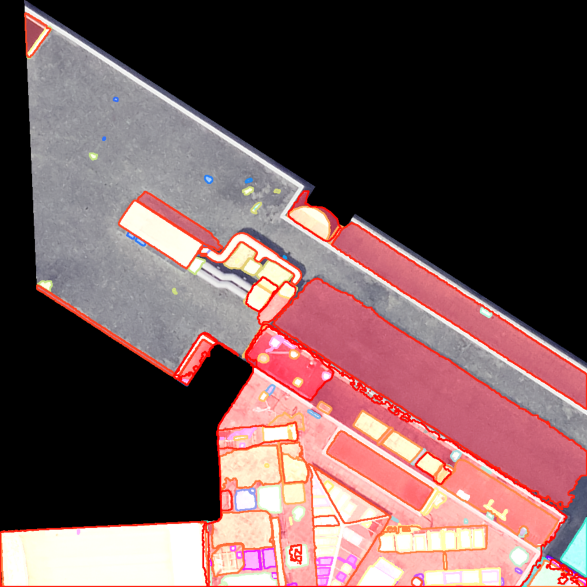
\includegraphics[width=\textwidth]{02-main/figures/ch3_essai_sam_05_filtered_masks_overlay.png}
        \caption{Mise en évidence des polygones filtrés}
        \label{fig:ch3_essai_sam_05_filtered_masks_overlay}
    \end{subfigure}
    \hfill
    \begin{subfigure}[b]{0.48\textwidth}
        \centering
        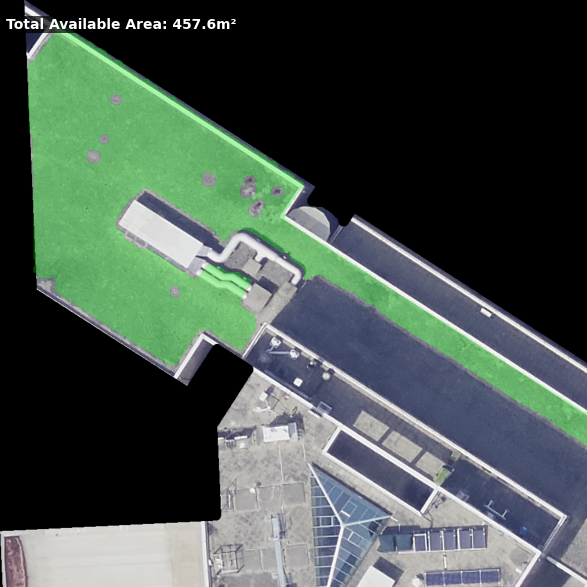
\includegraphics[width=\textwidth]{02-main/figures/ch3_essai_sam_06_une_zone_libre.png}
        \caption{Espace libre}
        \label{fig:ch3_essai_sam_06_une_zone_libre}
    \end{subfigure}

    \caption{Essai d'utilisation de SAM}
    \label{fig:essai_algo_sam}
\end{figure}

\subsubsection{Fine-tuning de SAM}
La piste d'un fine-tuning de SAM pour mieux l'adapter à la tâche d'identification des espaces libres a été explorée. Un dataset de 45 images (Figure \ref{fig:ch3_piste_exploree_classification_11_fine_tuning_dataset}) n'a pas permis d'améliorer significativement les performances du modèle. Une des problématiques rencontrées lors de la création de ce dataset est qu'il faut identifier tous les obstacles présents sur la toiture, ce qui prend énormément de temps et nécessite une grande quantité de classes différentes.

\begin{figure}[H]
    \centering
    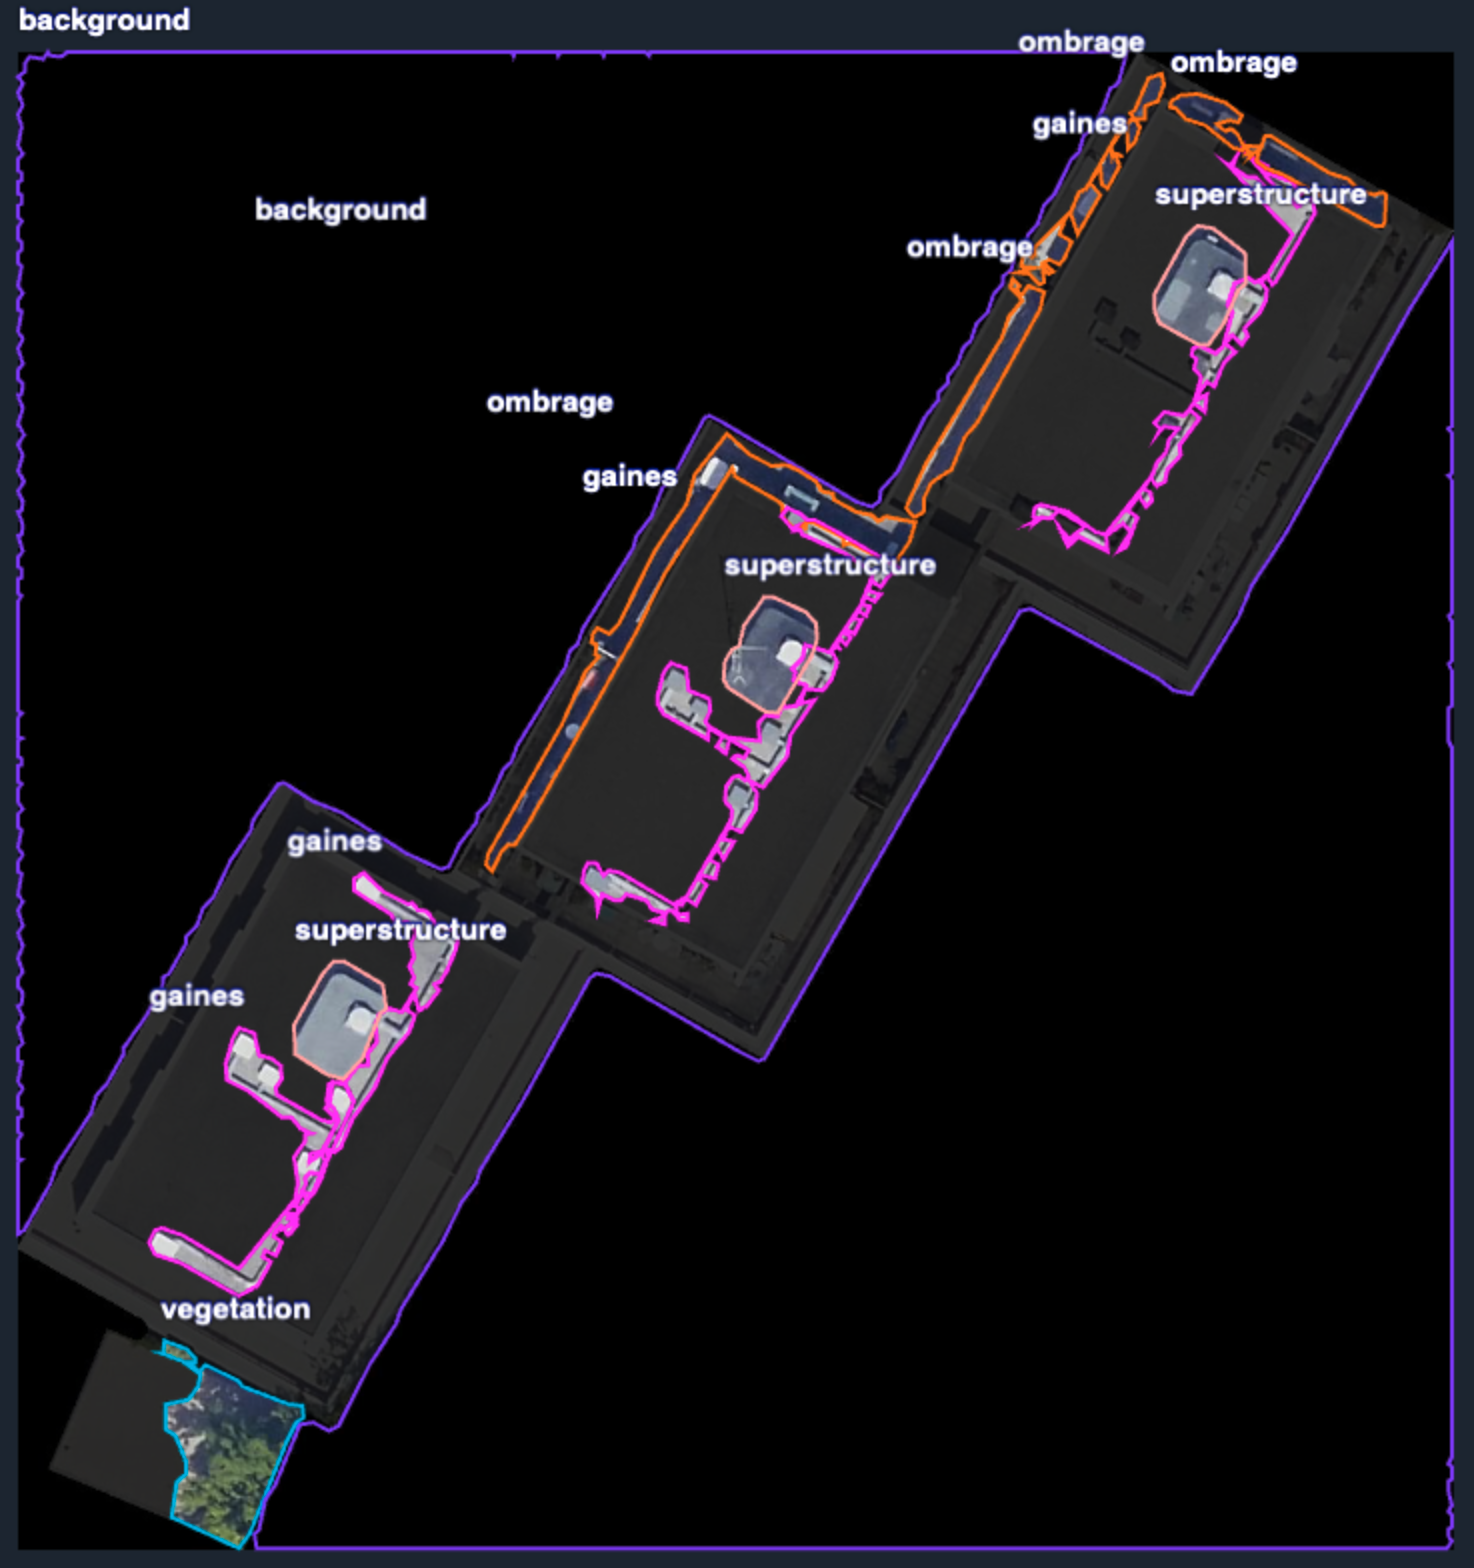
\includegraphics[width=1\linewidth]{02-main/figures/ch3_piste_exploree_classification_11_fine_tuning_dataset.png}
    \caption{Image du dataset pour le fine-tuning SAM}
    \label{fig:ch3_piste_exploree_classification_11_fine_tuning_dataset}
\end{figure}

\subsubsection{Résultats}

SAM segmente correctement les toitures bien éclairées avec un contraste suffisant entre obstacles et surface. Les résultats se dégradent significativement en présence d'ombrages ou de faible contraste.

Les principales limitations sont:
\begin{itemize}
    \item Principal problème rencontré sont les ombrages. SAM confond les zones ombragées avec l'arrière-plan noir, même avec les filtres de luminosité implémentés. Cela génère des faux négatifs dans les zones ombragées.
    \item Le temps de calcul par image est de 7 minutes (sur \acrshort{gpu}), ce qui confirme les résultats de \acrshort{stdl}. La mise à l'échelle du canton est problématique.
    \item Les performances de segmentation sont directement corrélées à la résolution et au contraste de l'image d'entrée.
\end{itemize}

Le fine-tuning avec 45 images annotées n'améliore pas les performances. Le dataset reste trop petit pour un modèle de cette complexité, et l'annotation manuelle de tous les obstacles de toiture est très chronophage.

Pour conclure, SAM fonctionne bien sur des images de qualité avec un bon éclairage, par contre son utilité reste limitée à cause des ombrages et du temps de calcul nécessaire.